% Options for packages loaded elsewhere
\PassOptionsToPackage{unicode}{hyperref}
\PassOptionsToPackage{hyphens}{url}
\PassOptionsToPackage{dvipsnames,svgnames,x11names}{xcolor}
%
\documentclass[
]{ccr}

% [WvA] change from original template.tex - amssymb is replaced by / clashes with newtxmath]
% \usepackage{amsmath,amssymb}
\usepackage{amsmath}

\usepackage{iftex}
\ifPDFTeX
  \usepackage[T1]{fontenc}
  \usepackage[utf8]{inputenc}
  \usepackage{textcomp} % provide euro and other symbols
\else % if luatex or xetex
  % [WvA] change from original template.tex - unicode-math is replaced by / clashes with newtxmath]
  %% \usepackage{unicode-math}
  \defaultfontfeatures{Scale=MatchLowercase}
  \defaultfontfeatures[\rmfamily]{Ligatures=TeX,Scale=1}
\fi
% Use upquote if available, for straight quotes in verbatim environments
\IfFileExists{upquote.sty}{\usepackage{upquote}}{}
\IfFileExists{microtype.sty}{% use microtype if available
  \usepackage[]{microtype}
  \UseMicrotypeSet[protrusion]{basicmath} % disable protrusion for tt fonts
}{}
\makeatletter
\@ifundefined{KOMAClassName}{% if non-KOMA class
  \IfFileExists{parskip.sty}{%
    \usepackage{parskip}
  }{% else
    \setlength{\parindent}{0pt}
    \setlength{\parskip}{6pt plus 2pt minus 1pt}}
}{% if KOMA class
  \KOMAoptions{parskip=half}}
\makeatother
\usepackage{xcolor}
\setlength{\emergencystretch}{3em} % prevent overfull lines
\setcounter{secnumdepth}{-\maxdimen} % remove section numbering
% Make \paragraph and \subparagraph free-standing
\ifx\paragraph\undefined\else
  \let\oldparagraph\paragraph
  \renewcommand{\paragraph}[1]{\oldparagraph{#1}\mbox{}}
\fi
\ifx\subparagraph\undefined\else
  \let\oldsubparagraph\subparagraph
  \renewcommand{\subparagraph}[1]{\oldsubparagraph{#1}\mbox{}}
\fi


\providecommand{\tightlist}{%
  \setlength{\itemsep}{0pt}\setlength{\parskip}{0pt}}\usepackage{longtable,booktabs,array}
\usepackage{calc} % for calculating minipage widths
% Correct order of tables after \paragraph or \subparagraph
\usepackage{etoolbox}
\makeatletter
\patchcmd\longtable{\par}{\if@noskipsec\mbox{}\fi\par}{}{}
\makeatother
% Allow footnotes in longtable head/foot
\IfFileExists{footnotehyper.sty}{\usepackage{footnotehyper}}{\usepackage{footnote}}
\makesavenoteenv{longtable}
\usepackage{graphicx}
\makeatletter
\def\maxwidth{\ifdim\Gin@nat@width>\linewidth\linewidth\else\Gin@nat@width\fi}
\def\maxheight{\ifdim\Gin@nat@height>\textheight\textheight\else\Gin@nat@height\fi}
\makeatother
% Scale images if necessary, so that they will not overflow the page
% margins by default, and it is still possible to overwrite the defaults
% using explicit options in \includegraphics[width, height, ...]{}
\setkeys{Gin}{width=\maxwidth,height=\maxheight,keepaspectratio}
% Set default figure placement to htbp
\makeatletter
\def\fps@figure{htbp}
\makeatother
\newlength{\cslhangindent}
\setlength{\cslhangindent}{1.5em}
\newlength{\csllabelwidth}
\setlength{\csllabelwidth}{3em}
\newlength{\cslentryspacingunit} % times entry-spacing
\setlength{\cslentryspacingunit}{\parskip}
\newenvironment{CSLReferences}[2] % #1 hanging-ident, #2 entry spacing
 {% don't indent paragraphs
  \setlength{\parindent}{0pt}
  % turn on hanging indent if param 1 is 1
  \ifodd #1
  \let\oldpar\par
  \def\par{\hangindent=\cslhangindent\oldpar}
  \fi
  % set entry spacing
  \setlength{\parskip}{#2\cslentryspacingunit}
 }%
 {}
\usepackage{calc}
\newcommand{\CSLBlock}[1]{#1\hfill\break}
\newcommand{\CSLLeftMargin}[1]{\parbox[t]{\csllabelwidth}{#1}}
\newcommand{\CSLRightInline}[1]{\parbox[t]{\linewidth - \csllabelwidth}{#1}\break}
\newcommand{\CSLIndent}[1]{\hspace{\cslhangindent}#1}

\usepackage{setspace} \usepackage{multirow} \usepackage{pdflscape} \usepackage{url} \makeatletter \renewcommand\tiny{\@setfontsize\tiny{7.5}{8}} \renewcommand\small{\@setfontsize\small{8.5}{10}} \makeatother
\makeatletter
\makeatother
\makeatletter
\makeatother
\makeatletter
\@ifpackageloaded{caption}{}{\usepackage{caption}}
\AtBeginDocument{%
\ifdefined\contentsname
  \renewcommand*\contentsname{Table of contents}
\else
  \newcommand\contentsname{Table of contents}
\fi
\ifdefined\listfigurename
  \renewcommand*\listfigurename{List of Figures}
\else
  \newcommand\listfigurename{List of Figures}
\fi
\ifdefined\listtablename
  \renewcommand*\listtablename{List of Tables}
\else
  \newcommand\listtablename{List of Tables}
\fi
\ifdefined\figurename
  \renewcommand*\figurename{Figure}
\else
  \newcommand\figurename{Figure}
\fi
\ifdefined\tablename
  \renewcommand*\tablename{Table}
\else
  \newcommand\tablename{Table}
\fi
}
\@ifpackageloaded{float}{}{\usepackage{float}}
\floatstyle{ruled}
\@ifundefined{c@chapter}{\newfloat{codelisting}{h}{lop}}{\newfloat{codelisting}{h}{lop}[chapter]}
\floatname{codelisting}{Listing}
\newcommand*\listoflistings{\listof{codelisting}{List of Listings}}
\makeatother
\makeatletter
\@ifpackageloaded{caption}{}{\usepackage{caption}}
\@ifpackageloaded{subcaption}{}{\usepackage{subcaption}}
\makeatother
\makeatletter
\@ifpackageloaded{tcolorbox}{}{\usepackage[skins,breakable]{tcolorbox}}
\makeatother
\makeatletter
\@ifundefined{shadecolor}{\definecolor{shadecolor}{rgb}{.97, .97, .97}}
\makeatother
\makeatletter
\makeatother
\makeatletter
\makeatother
\ifLuaTeX
  \usepackage{selnolig}  % disable illegal ligatures
\fi
\IfFileExists{bookmark.sty}{\usepackage{bookmark}}{\usepackage{hyperref}}
\IfFileExists{xurl.sty}{\usepackage{xurl}}{} % add URL line breaks if available
\urlstyle{same} % disable monospaced font for URLs
\hypersetup{
  pdftitle={How COVID-19 and the News Shaped Populism in Facebook Comments in Seven European Countries. A Computational Analysis.},
  pdfauthor={Daniel Thiele},
  pdfkeywords={populism, COVID-19, social media, multilingual,
computational text analysis, word embeddings, user comments},
  colorlinks=true,
  linkcolor={blue},
  filecolor={Maroon},
  citecolor={Blue},
  urlcolor={Blue},
  pdfcreator={LaTeX via pandoc}}

\title{How COVID-19 and the News Shaped Populism in Facebook Comments in
Seven European Countries. A Computational Analysis.}
\authorsnames{Daniel Thiele}
\authorsaffiliations{
    {Freie Universität Berlin, Weizenbaum Institute Berlin}
}


\begin{document}
\abstract{Citizen-generated populism is flourishing in the comments
sections of online news. The factors that shape the extent of such
populist communication from below are still under-researched. This study
focuses on the COVID-19 crisis to examine how contextual and
media-related factors are related to the extent of populism in comment
sections on Facebook pages of news outlets from seven European countries
(AT, DE, FR, IT, NL, SE and UK). Computational text analysis, machine
translation and Bayesian multilevel regression were used to analyze
digital trace data from 65,258 posts and 3.4 million comments published
between February 2020 and June 2021. The computational measurements -
multilingual dictionaries for posts and distributed dictionary
representation to capture populism in comments - were rigorously
validated. The results show that posts referring to the government,
experts, COVID-19, and restrictions exhibit higher levels of populism in
the comments sections. The stringency of containment policies was
positively associated with populism in Germany, Austria, and the
Netherlands when COVID-19 was mentioned. Lower levels of populism were
observed for tabloid media and when news outlets engaged in visible
moderation. The implications of these findings beyond the pandemic
context and methodological challenges are discussed.}
\keywords{populism, COVID-19, social media, multilingual, computational
text analysis, word embeddings, user comments}
\maketitle
\volume{0}
\pubnumber{0}
\pubyear{2024}
\firstpage{1}
\doi{10.5117/CCR2024.TBA}
\shortauthors{Thiele}\ifdefined\Shaded\renewenvironment{Shaded}{\begin{tcolorbox}[sharp corners, interior hidden, breakable, boxrule=0pt, frame hidden, enhanced, borderline west={3pt}{0pt}{shadecolor}]}{\end{tcolorbox}}\fi

\hypertarget{introduction}{%
\subsection{Introduction}\label{introduction}}

Populist messages travel well on social media (Ernst et al. 2019;
Gerbaudo 2018). Politicians employ populist communication to stimulate
user interactions (Jost, Maurer, and Hassler 2020). The participatory
logic of social media also allows ordinary citizens to express their
populist views (de Vreese et al. 2018). Comments sections below news are
bursting with citizen-generated populism, whether on websites (Blassnig,
Engesser, et al. 2019) or on Facebook pages operated by news media
(Thiele 2022a). In parallel to a growing interest in populist attitudes
(Marcos-Marne, Gil de Zúñiga, and Borah 2023), researchers have begun to
investigate populism in user comments (e.g., Blassnig, Engesser, et al.
2019; Galpin and Trenz 2019). These studies have focused on election
periods (Blassnig, Engesser, et al. 2019; Galpin and Trenz 2019) or
relied on narrow country selections (Thiele 2022a). What is lacking are
cross-national studies that provide a comprehensive understanding of how
``populism in reader comments is influenced by characteristics of the
article or other context factors'' (Blassnig, Ernst, et al. 2019, 1124).
This study narrows this research gap by examining populism in user
comments (henceforth ``comments'') on news media Facebook pages from
seven European countries -- Austria, France, Germany, Italy,
Netherlands, Sweden, and the United Kingdom -- in the context of
COVID-19.

COVID-19 provides a unique opportunity for studying contextual
influences on citizen-generated populism. Government containment
policies drastically restricted personal freedoms, triggering
psychological reactance in some citizens (Dillard et al. 2023). In many
European countries, containment policies were met with protests (Kriesi
and Oana 2023; Neumayer, Pfaff, and Plümper 2023) that resonated with
populist ideology (Brubaker 2021; Stecula and Pickup 2021). Expressing
discontent online became increasingly important during lockdowns (Kriesi
and Oana 2023). Online, COVID-19 was accompanied by an ``infodemic'',
which is particularly well researched with regard to the spread of
conspiracy theories (Righetti, Rossi, and Marino 2022). Less is known
about the crisis's impact on the proliferation of populist content in
comments sections, which is unfortunate as comments can, for instance,
influence other readers' attitudes toward vaccinations (Sun and Lu
2023). Previously, I found that populist comments in Germany and Austria
are linked to media coverage of COVID-19 (Thiele 2022a). The limited
country selection of that study prevented an adequate investigation of
the impact of containment policies and additional media-related factors.
Addressing these shortcomings, the present study aims to answer the
following research question: How did the COVID-19 crisis and
media-related factors influence populism in user comments on news media
Facebook pages in seven Western European countries?

Here, seven hypotheses and three research questions are examined using
digital trace data. This data source warrants high external validity
(Blassnig, Engesser, et al. 2019, 630) but does not allow the direct
testing of psychological mechanisms. Therefore, the analysis focuses on
the contextual correlates of populism in user comments. A total of
65,258 posts and 3.4 million comments posted during the first three
waves of COVID-19 (February 2020 -- June 2021) on 21 news media Facebook
pages from seven European countries (AT, DE, FR, IT, NL, SE, UK) was
analyzed. Comments were machine-translated (Vries, Schoonvelde, and
Schumacher 2018) into German. To measure populism, a computational text
analysis technique called ``distributed dictionary representation''
(Garten et al. 2018) was implemented (Thiele 2022b), applied, and
validated. Post characteristics were captured using validated
multilingual dictionaries. Real-world data were obtained from the Oxford
COVID-19 government response tracker (OxCGRT) (Hale et al. 2020).
Hypotheses were tested using Bayesian multilevel linear regression
models (Bürkner et al. 2022).

The results show that Facebook posts mentioning the government, experts,
COVID-19, and restrictions were associated with higher levels of
populism in comments. The stringency of COVID-19 policies affected
populism differently in the analyzed countries. I found a limited,
positive association in Germany, Austria, and the Netherlands when posts
mentioned COVID-19. Moderating comments by the media and, surprisingly,
the media-type tabloid press were associated with lower levels of
populism. The study concludes by discussing the implications of the
findings beyond the pandemic and methodological limitations.

\hypertarget{theory}{%
\subsection{Theory}\label{theory}}

\hypertarget{populism-in-user-comments}{%
\subsubsection{Populism in User
Comments}\label{populism-in-user-comments}}

Social media has changed the logic of political communication,
integrating ordinary citizens into producing and distributing the news
(Klinger and Svensson 2015). Most news media outlets operate pages on
social media, where they share links to articles on their websites.
Facebook remains the most widely used social media platform for news
consumption in all countries studied here, although its heyday has
passed (Newman et al. 2022). On Facebook, users can comment under posts
to express their opinions and engage in discussions and deliberation
(Dahlberg 2011) or for less constructive purposes (Quandt 2018).
Negative aspects, such as high levels of incivility, often prevail in
these spaces (Coe, Kenski, and Rains 2014). Populist content is one of
those negative aspects (Waisbord 2018) and can have detrimental
implications for the quality of the user discussion (Thiele and Turnšek
2022).

Following Mudde (2004, 543), populism is a thin-centered ideology which
holds that `the people' are ruled by a `corrupt elite' and which demands
unrestricted popular sovereignty. Populists imagine the people as a
``homogenous and virtuous community'' (Hawkins and Rovira Kaltwasser
2018, 3) that is only divided and deprived of its sovereignty at the
instigation of a treacherous elite (Mudde 2004). The concept entails at
least two dimensions: \emph{anti-elitism} and \emph{people-centrism}
(Rooduijn 2019). Popular sovereignty, which is sometimes considered a
third dimension, is here considered as the point of contention between
the people and the elite (Aslanidis 2018, 1255). Following a
communication-centered approach, I focus on expressions of populist
ideas in text (de Vreese et al. 2018). Online, populist ideology is
often communicated in fragments (Engesser et al. 2017). Messages can be
therefore more or less populist on a continuous scale (Aslanidis 2018).
Different actors can disseminate populist messages. Populism from
politicians (Ernst et al. 2019) and journalists (Wettstein et al. 2019)
has received most scholarly attention. Although populism revolves around
the idea of making the people's voice heard (Canovan 1999), only a
handful of studies have focused on populist content disseminated by
ordinary citizens (Blassnig, Engesser, et al. 2019; Blassnig, Ernst, et
al. 2019; Galpin and Trenz 2019; Thiele 2022a; Thiele and Turnšek 2022).
These studies have mostly analyzed comments on news websites (Blassnig,
Engesser, et al. 2019; Galpin and Trenz 2019). Here, I focus on comments
below news media posts on Facebook, which is a preferred social media
platform among populists (Schulz 2019). Facebook comments also exhibit a
particularly low deliberative quality (Esau, Friess, and Eilders 2017).

To explain the occurrence of populist comments, Blassnig et al. (2019,
634) have suggested to consider them as expressions of populist
attitudes. Following Hawkins et al. (2020), populist attitudes require
activation through the political context. Krämer (2014, 55) argued that
messages, such as media coverage, can activate a cognitive ``populism
schema'' through priming. Hameleers et al. (2021) showed that fragments
of populist communication can activate larger clusters of populist
attitudes. Here, I argue that mentioning representatives of the elite in
media posts works as an activating cue that eventually triggers populist
comments. The elite is the key antagonist for populists (Hameleers et
al. 2021). Governments and experts are frequent targets of populist
rhetoric (Jagers and Walgrave 2007; Mede and Schäfer 2020) and were
omnipresent in media coverage as managers of the COVID-19 crisis
(Brubaker 2021). Mentioning these groups may activate populist attitudes
and motivate populist citizens to express these views, possibly by an
emotional mechanism (Rico, Guinjoan, and Anduiza 2017). Previous
findings support this argument (Thiele 2022a). Therefore, I hypothesize
the following:

\textbf{H1:} Facebook posts from news media mentioning the government
are associated with increased levels of populism in the comments
section.

\textbf{H2:} Facebook posts from news media mentioning experts are
associated with increased levels of populism in the comments section.

Second, newsrooms' practices in moderating comments might affect opinion
expression (Gibson 2019). Some moderation practices are visible to other
users, for example, when news media pages comment below their own posts
to remind users about conversational rules (Wintterlin et al. 2020).
Populist users, known for breaching such norms (Hameleers 2019), may
react to such moderation by turning silent, as they sense a hostile
opinion climate (Matthes, Knoll, and von Sikorski 2018). Conversely,
moderation might also backfire if it is perceived as censorship
(Sherrick and Hoewe 2018). Against this backdrop, I pose the following
open research question regarding comments authored by the news media
pages themselves:

\textbf{RQ1:} How are comments from news media moderating discussions on
Facebook associated with the level of populism in comments sections?

Third, the level of populism in comments sections may vary across the
type of news media operating the Facebook page. Theorists have often
claimed complicity between the tabloid press and populism (Krämer 2014;
Mazzoleni 2008), but content analyses have struggled to corroborate this
claim (e.g., Bos and Brants 2014). Readers of tabloid newspapers,
however, support populist attitudes more strongly than audiences of
public television or quality press (Schulz 2019). The implications of
these findings for populism in comments remain unclear. Hence, I pose a
second open research question:

\textbf{RQ2:} How is the type of news media operating a Facebook page
associated with the level of populism in comments sections?

\hypertarget{the-pandemic-and-populism}{%
\subsubsection{The Pandemic and
Populism}\label{the-pandemic-and-populism}}

One main objective of this study is to examine how the context of
COVID-19 has affected populism in comments. COVID-19 yielded a range of
political consequences. While the first wave saw increased support for
governments (Schraff 2021), later stages were characterized by growing
polarization and protests against containment policies (Kriesi and Oana
2023; Neumayer, Pfaff, and Plümper 2023). Scholars have linked those
protests to populist ideology (Brubaker 2021; Flew 2021; Stecula and
Pickup 2021). Both, protesters against COVID-19 containment policies and
populists exhibit a fundamental distrust in elites, an appetite for
conspiracy theories, and a preference for commonsensical over expert
knowledge (Brubaker 2021; Stecula and Pickup 2021). Populist parties in
Europe did not respond uniformly to the outbreak of the pandemic
(Wondreys and Mudde 2022) but tried to later capitalize on the protests.
Previous research has explained these protest events by strategic
considerations of the organizers (Neumayer, Pfaff, and Plümper 2023).
This explanation is convincing for offline events but offers little to
explain expressions of discontent online, where little collective
organization is required. The argument proposed here instead draws on a
psychological mechanism.

\emph{Psychological reactance} (J. W. Brehm 1966; S. S. Brehm and Brehm
1981) provides a conceptual framework to link the COVID-19 crisis and
expressions of populism\emph{.} Reactance ``is the motivational state
that is hypothesized to occur when a freedom is eliminated or
threatened'' (S. S. Brehm and Brehm 1981, 37). It involves anger and
negative cognitions motivating people to restore the threatened freedom
or, if this option is blocked, to engage in aggressive or compensatory
behavior (Dillard and Shen 2005; Rosenberg and Siegel 2018). Cumulative
evidence shows that the severity of a restriction tends to increase
reactance (Rosenberg and Siegel 2018, 3). While individuals react
differently to experiencing reactance, commonly observed responses are
expressing hostility toward, and derogating the source of, the
restriction (Rosenberg and Siegel 2018, 3). COVID-19 containment
policies triggered such reactance reactions in some individuals (Dillard
et al. 2023).

I argue that experiencing reactance can activate populist attitudes
(Hawkins, Rovira Kaltwasser, and Andreadis 2020) because of the anger
involved in it (Dillard and Shen 2005). Anger has been linked to the
support of populist ideas (Rico, Guinjoan, and Anduiza 2017), and
experiencing reactance during COVID-19 is associated with
anti-government attitudes (Hajek and Häfner 2021). Moreover, populist
expressions by opponents of containment policies reflect what reactance
researchers call derogating the source of the restriction (Rosenberg and
Siegel 2018). For example, the government, scientists, and the media are
denounced for having fabricated the crisis to impose a dictatorship
(Brubaker 2021). While examining individual motivations for such
statements is beyond the scope of this study, the theoretical framework
sketched here is useful for deriving hypotheses regarding the impact of
contextual (Hawkins, Rovira Kaltwasser, and Andreadis 2020) and
content-based (Krämer 2014) factors on populism in comments.

First, reactance occurs more frequently when people believe they are
being targeted by persuasion (Rosenberg and Siegel 2018). Media coverage
of COVID-19 arguably included fear appeals (Sun and Lu 2023; Thiele
2022a) that is ``persuasive messages designed to scare people by
describing the terrible things that will happen to them if they do not
do what the message recommends'' (Witte 1992, 329). Opponents of
COVID-19 policies often suspect COVID-19 coverage to be propaganda (Flew
2021). Those citizens believe themselves to be targeted by a persuasion
campaign. Such beliefs should spark reactance and could motivate
citizens to express their anger in comments. Previous findings linked
COVID-19 coverage in Germany and Austria to populist comments (Thiele
2022a). News posts that explicitly mention restrictive COVID-19 policies
may provoke even stronger reactions, as they prime freedom-threatening
aspects. Following these considerations, I hypothesize the following:

\textbf{H3}: Facebook posts from news media mentioning COVID-19 are
associated with increased levels of populism in the comments section.

\textbf{H4}: Facebook posts from news media mentioning restrictive
COVID-19 containment policies are associated with increased levels of
populism in the comments section.

Second, the magnitude of the threat to personal freedoms has been
repeatedly found to be positively related to the level of reactance
(Organ 1974; Rosenberg and Siegel 2018). In the context of COVID-19, the
magnitude of restrictions can be determined as the ``stringency'' of
COVID-19 containment policies, which included lockdowns, closing public
venues, travel restrictions, or obligations to wear masks. To be clear,
stringency denotes the severity of COVID-19 containment policies varying
by day and country (Hale et al. 2020), \emph{not} the logical
consistency of policies. Additionally, I expect that the stringency of
COVID-19 policies affects populism in comments sections only if the news
post mentions the topic of COVID-19. Therefore, I hypothesize:

\textbf{H5}: For Facebook posts from news media mentioning COVID-19, the
stringency of COVID-19 containment policies is associated with increased
levels of populism in the comments section.

Third, the \emph{stringency} of containment policies varied considerably
in the countries studied here (Gordon, Grafton, and Steinshamn 2021).
Italy, for example, was hit early and hard by the pandemic and imposed
tough restrictions, while Sweden followed a laissez-faire approach. The
restrictions in Germany and France were comparable but the protests
differed widely (Kriesi and Oana 2023). How these patterns translate to
populist expressions online remains unclear. Hence, I pose the
explorative research question:

\textbf{RQ3:} How does the association between stringency of COVID-19
containment policies and the level of populism in comments sections vary
by country?

Finally, drawing on previous findings (Jørgensen et al. 2022, 1), I
expect that a ``pandemic fatigue'' increased levels of political
discontent and expressions of populist attitudes over time. One reason
could be that repeating persuasive messages can increase reactance (Koch
and Zerback 2013). Similarly, message novelty has been linked to less
reactance (Rosenberg and Siegel 2018). The former implies an effect that
gradually increases over time, while the latter suggests considerably
lower levels of populism during the first wave of COVID-19. Similar
associations were observed previously (Thiele 2022a). As a result, I
hypothesize the following:

\textbf{H6}: Throughout the COVID-19 crisis, the level of populism in
comments sections increased.

\textbf{H7}: During the first wave of the COVID-19 crisis, the level of
populism in comments sections was lower, compared to later stages.

\hypertarget{data-and-methods}{%
\subsection{Data and Methods}\label{data-and-methods}}

\hypertarget{data}{%
\subsubsection{Data}\label{data}}

This study analyzes digital trace data, downloaded via Facebook API
using Facepager (Jünger and Keyling 2020) and R. These data warrant high
external validity, as they trace behavior that is likely to be
suppressed in experiments due to social desirability (Blassnig,
Engesser, et al. 2019, 630). Anonymization through the API, however,
limits individual-level analysis. Hence, this study analyzes the
correlates of populism in comments but cannot test psychological or
causal mechanisms directly.

The country selection aimed at maximizing variance in the stringency of
containment policies and the scope of protests (Neumayer, Pfaff, and
Plümper 2023). Seven European countries were selected: Austria (AT),
Germany (DE), France (FR), Italy (IT), Netherlands (NL), Sweden (SE),
and United Kingdom (UK). These countries varied considerably regarding
the stringency of COVID-19 containment policies and the level of
protests against them (Neumayer, Pfaff, and Plümper 2023).

\newpage
{
\begin{spacing}{.9}
\fontsize{9}{10}\selectfont 
\begin{longtable}[]{@{}
  >{\raggedright\arraybackslash}p{.1\linewidth}
  >{\raggedright\arraybackslash}p{.25\linewidth}
  >{\raggedright\arraybackslash}p{.18\linewidth}
  >{\raggedleft\arraybackslash}p{.17\linewidth}
  >{\raggedleft\arraybackslash}p{.15\linewidth}@{}}
\caption{Selected News Media Facebook Pages}\tabularnewline
\toprule\noalign{}
\textbf{Country} & \textbf{Facebook page} & \textbf{Type} & \textbf{Follower (n)} & \textbf{Posts (n)} \\
\midrule\noalign{}
\endhead
\bottomrule\noalign{}
\endlastfoot
AT & Der Standard & Quality & 316,613 & 4,094 \\
\multicolumn{1}{c}{\centering } &   Kronen Zeitung & Tabloid & 360,190 &    5,334 \\
\multicolumn{1}{c}{\centering } &   Zeit im Bild &  Public broadcaster &    807,049 &   2,917 \\
DE  & Der Spiegel   & Quality   & 1,922,150 &   3,010 \\
\multicolumn{1}{c}{\centering } &   Bild &  Tabloid & 2,545,380 &   3,598 \\
\multicolumn{1}{c}{\centering } &   Tagesschau &    Public broadcaster &    1,966,320 &  3,458 \\
FR  & Le Monde &    Quality & 4,661,594 &   2,873 \\
\multicolumn{1}{c}{\centering } &   20 Minutes &    Tabloid & 2,968,467 &   2,891 \\
\multicolumn{1}{c}{\centering } &   Franceinfo &    Public broadcaster &    1,987,567 & 3,054 \\
IT &    La Repubblica   & Quality   & 3,969,463 &   2,891 \\
\multicolumn{1}{c}{\centering } &   Tgcom24 & Tabloid   & 2,344,620 &   2,693 \\
\multicolumn{1}{c}{\centering } &   Rainews.it  & Public broadcaster &  528,740 &   2,963 \\
NL &    De Telegraaf &  Quality &   512,635 &   3,037 \\
\multicolumn{1}{c}{\centering } &   AD.nl & Tabloid & 557,329 & 3,743 \\
\multicolumn{1}{c}{\centering } &   NOS &   Public broadcaster &    935,907 &   3,133 \\
SE &    Aftonbladet & Quality & 505,268 &   2,721 \\
\multicolumn{1}{c}{\centering } &   Dagens Nyheter &    Tabloid & 216,073 & 3,194 \\
\multicolumn{1}{c}{\centering } &   SVT Nyheter &   Public broadcaster &    204,169 &   3,208 \\
UK &    The Guardian &  Quality &   8,469,271 &  2,889 \\
\multicolumn{1}{c}{\centering } &   Daily Mail &    Tabloid & 16,643,114 &  1,848 \\
\multicolumn{1}{c}{\centering } &   BBC News &  Public broadcaster &    53,516,028 &    1,709 \\
\midrule\noalign{}
\textbf{Total} & & & & \textbf{65,258} \\
\end{longtable}
\end{spacing}
}

These countries also represent different (legacy) media systems (Hallin
and Mancini 2004). What all seven countries have in common is that they
are liberal, Western European democracies that have a record of
successful mobilization by populist parties, mostly from the right
(Mudde 2007). Per country, I selected one news media outlet for each of
the three media types quality press, tabloid press, and public
broadcaster, based on the weekly reach of the corresponding news website
(Newman et al. 2022). For each outlet, I identified the corresponding
Facebook page. Data were only collected from Facebook. Table 1 reports
the selected outlets by country and media type, along with the number of
Facebook followers, and the number of posts considered in the analysis.

From each Facebook page, all accessible posts published in the first
three waves of COVID-19 (1 February 2020 -- 30 June 2021) were
downloaded. For each of the n=65,258 posts, the first 100 comments were
downloaded, resulting in a dataset of n=3,424,691 comments. Capping the
number of comments aimed to limit the number of API calls, as the access
is shared with all Facepager users (Jünger and Keyling 2020). The cap is
ten times larger than in previous studies (Blassnig, Engesser, et al.
2019, 636), and higher than the median number of comments per post
(n=58).

\hypertarget{validation-data}{%
\subsubsection{Validation Data}\label{validation-data}}

For validation, 2,040 posts and 2,040 comments were randomly sampled
with equal distribution across countries for annotation by six
native-speaking, trained coders (five students and the author); 150
units each were machine-translated for parallel coding. Reliability is
reported as Krippendorff's alpha. Occurrences of \emph{anti-elitism}
(alpha=.80) and \emph{people-centrism} (.73) were coded binarily in
comments. Considering the fragmentary nature of populist online
communication (Engesser et al. 2017), a comment was considered populist
if either people-centrism or anti-elitism was coded. Posts were coded
for references to \emph{COVID-19} (.96), \emph{restrictive containment
policies} (.75), the \emph{government} (.78), and scientific
\emph{experts} (.76). The instructions align with Blassnig, Engesser, et
al. (2019; see also Blassnig, Engesser, and Esser 2016) and a previously
used codebook (Thiele 2022a) and are documented in Appendix A.

\hypertarget{multilingual-data}{%
\subsubsection{Multilingual Data}\label{multilingual-data}}

Computational analyses of multilingual texts face the challenge of
ensuring measurement equivalence and context-sensitivity across
countries, while maintaining cost-efficiency (Licht and Lind 2023).
Formal criteria for the first two aspects have yet to be established
(Licht and Lind 2023). Here, several strategies were used to approach
these goals. Relying on native speakers to annotate the validation data
was a first step. The further procedure differed for posts and comments.

Multilingual dictionaries were used to capture topics and actors
mentioned in posts. Dictionaries count the occurrence of keywords.
Pretests suggested that high levels of recall\emph{,} indicating
performance in capturing all relevant documents, and precision,
indicating performance in capturing only relevant documents, could be
achieved by translating an existing German dictionary (Thiele 2022a).
This was the most cost-effective solution. The dictionary was translated
using in-context translation websites (context.reverso.net; linguee.de).
The country-specific dictionaries were expanded by nearest neighbors
from word embeddings (\emph{fastText}) (Bojanowski et al. 2017), trained
on post data. Word embeddings represent semantic relations of words in a
vector space and result from machine learning algorithms, trained on
large corpora (e.g., Bojanowski et al. 2017). With the help of the
mentioned translation websites, I identified and removed terms that
tapped into unintended contexts. Validation is reported in the section
on explanatory variables.

For capturing populism in comments, translating an existing German
dictionary (Gründl 2022) was deemed not feasible, as it contains 13k
regular expressions. To find a ``common denominator'' for comparison,
comments were machine-translated (Licht and Lind 2023, 9). Following
findings of Vries et al. (2018), I opted for the Google Translate API.
German was chosen as the lingua franca, as this limited the costs most
efficiently and matched my expertise in capturing populism in German
text (Thiele and Turnšek 2022). For economic reasons, comments were
truncated to 540 characters before translation, which affected 1.8\% of
all comments.

Two further measures aimed at facilitating context-sensitivity and
equivalence. First, the translated corpus was used to train a custom
word embedding model, which underpins the populism measurement described
below. This model thus provides a common reference point, but also
accounts for country-specific uses of words that may persist even after
translation (Licht and Lind 2023, 23). Second, during optimization, I
selected the measurement that most coherently maximized the
output-validity score across countries. Despite these precautions, the
achieved level of equivalence is not perfect, as discussed in the next
and the concluding section.

\hypertarget{dependent-variable}{%
\subsubsection{Dependent Variable}\label{dependent-variable}}

Populism in comments was measured using the computational text analysis
technique ``distributed dictionary representation'' (DDR) (Garten et al.
2018). DDR combines dictionaries with word embeddings to measure how
strongly a concept is represented in a text (Garten et al. 2018).
Conventional dictionary approaches suffer from low recall (Rauh 2018).
DDR is similarly theory-driven as a dictionary, since it captures a
concept by researcher-defined keywords. However, it circumvents the need
to provide exhaustive lists of words by leveraging word embeddings. The
conceptual dictionary and each document are represented as average
vectors of the embeddings that represent the meaning of each word in
them. DDR then computes the cosine similarity between these vectors,
which can range from -1 to +1. This provides a crude indicator for how
strongly the concept is reflected in each document (Garten et al. 2018).
This technique works best with short, clear-cut dictionaries (Garten et
al. 2018, 348). The \emph{dictvectoR} (Thiele 2022b) R-package
implements DDR using \emph{fastText} word embeddings, which are tailored
to social media texts, and account for misspellings, out-of-vocabulary
words, and morphological rich languages, like German (Bojanowski et al.
2017). A custom \emph{fastText} model was trained on the translated and
originally German corpus of comments, and all German-speaking posts. The
model has 200 dimensions and a vocabulary of 89k words.

The populism measurement was optimized using 70\% of the annotated
comments, keeping 30\% as test sample. For evaluation, DDR scores were
transformed into binary predictors using logistic regression and
compared to the annotation. This is not a gold standard test but
circumvents the problem of producing granular manual annotations
reliably (Grimmer and Stewart 2013, 275). Evaluation focused on F1, a
harmonic mean of recall and precision. The optimization aimed to arrive
at a short, expressive dictionary that is \emph{inductive}
(i.e.~reflects the content of observed comments), \emph{theory-driven}
(i.e.~covers key dimensions of populism), and \emph{comparable}
(i.e.~maximizes F1 consistently across all countries). The process,
documented in Appendix C, followed the following steps: (a) identifying
words from the \emph{fastText} model's vocabulary that semantically
resemble the corpus annotated as populist; (b) adding
multiword-expressions; (c) manually selecting words on theoretical
grounds; (d) generating 2.9 million keyword combinations of different
lengths from these words; and (e) evaluating these dictionaries across
countries.

The dictionary that maximized F1 best across all countries is presented
in Table 1, along with translation and performance scores for the test
and train data. This dictionary was deemed theoretically convincing as
it features words that represent ``the elite'' from different areas of
society (\emph{``politics and media'', ``government'', ``nepotism'',}
\emph{``so-called experts'',} and \emph{''state media''}), words that
invoke ``the people'' as an in-group (``\emph{people'', ``taxpayers'',
``our system'',} and \emph{``our tax money''}), and words that
characterize the struggle over sovereignty between these antagonists
(``\emph{dictatorship'', ``muzzled'',} and \emph{``obfuscate''}).
Although these words are not necessarily populist in isolation, their
combined meaning cuts through a broad range of populist key messages
(Blassnig, Engesser, et al. 2019, 638). This short dictionary is
sensitive to the context of COVID-19 but should be able to capture
populism in other contexts as well.

{
\begin{spacing}{1}
\fontsize{9}{10}\selectfont
\begin{longtable}[]{@{}
  >{\raggedright\arraybackslash}p{.275\linewidth}
  >{\raggedright\arraybackslash}p{.275\linewidth}
  >{\centering\arraybackslash}p{.065\linewidth}
  >{\raggedleft\arraybackslash}p{.04\linewidth}
  >{\raggedleft\arraybackslash}p{.04\linewidth}
  >{\raggedleft\arraybackslash}p{.04\linewidth}
  >{\raggedleft\arraybackslash}p{.04\linewidth}@{}}
\caption{\label{tbl-ddr}Performance of DDR Measurement of Populism}\tabularnewline
\toprule\noalign{}
\textbf{Dictionary} & \textbf{Translation} & \textbf{Country} & \multicolumn{2}{c}{\textbf{n}} & \multicolumn{2}{c}{\textbf{F1}} \\
& & & \emph{Train} & \emph{Test} & \emph{Train} & \emph{Test} \\
\midrule\noalign{}
\endhead
%\bottomrule\noalign{}
\endlastfoot
\multirow{8}{*}{\shortstack[l]{\small\emph{'diktatur,’ ‘mundtot,’} \\
                               \small\emph{‘politik und medien,’} \\
                               \small\emph{‘regierung,’ ‘sogenannten } \\
                               \small\emph{experten,’ ‘staatsmedien,’} \\
                               \small\emph{‘steuerzahler,’ ‘unser } \\
                               \small\emph{system,’ ‘unsere steuer-} \\
                               \small\emph{gelder,’ ‘verschleiern,’} \\
                               \small\emph{‘vetternwirtschaft,’ ‘volk’} 
                               }} &
\multirow{8}{*}{\shortstack[l]{\small\emph{'dictatorship,' ‘muzzled’,} \\
                               \small\emph{‘politics and media’,} \\
                               \small\emph{‘government’, ‘so-called} \\
                               \small\emph{experts’, ‘state media’,} \\
                               \small\emph{‘taxpayers’, ‘our system’,} \\
                               \small\emph{‘our tax money’,} \\
                               \small\emph{‘obfuscate’, ‘nepotism’,} \\
                               \small\emph{‘people’}}}
                                                          & AT & 207 & 88 & .80 & .77 \\
                                                          & & DE & 213 & 90 & .76 & .80 \\
                                                          & & FR & 205 & 87 & .69 & .76 \\
                                                          & & IT & 199 & 84 & .71 & .71 \\
                                                          & & NL & 202 & 86 & .71 & .66 \\
                                                          & & SE & 200 & 85 & .70 & .74 \\
                                                          & & UK & 206 & 88 & .68 & .72 \\ \cline{3-7}
& & \textbf{All} & 1,432 & 608 & .73\textsuperscript{a} & \textbf{.74}\textsuperscript{b} \\
\midrule\noalign{}
\multicolumn{7}{l}{\tiny{\emph{Notes:} (a) Train -- Recall .73, Precision .72; (b) Test -- Recall .76, Precision .72}} \\
\end{longtable}
\end{spacing} 
}

The DDR measurement performs well overall (F1=.74) and is relatively
consistent across countries. It outperforms Gründl's (2022) dictionary,
which reached a low F1 of .19. Against this backdrop, I consider this
measurement a satisfactory proxy for populism. However, the
output-validity scores vary across countries, with the lowest
test-performance for the Netherlands (F1=.66), indicating a lack of
equivalence and measurement error differential to language. I account
for this by centering the populism scores on the country-level means. In
the concluding section I discuss the limitations of this approach.

The DDR measure was applied to the dataset of translated comments.
Titles of hyperlinks were used when comments contained no other text.
Text cleaning is documented in Appendix B. I replaced n=19,047 missing
values (0.6\%) by the mean populism score per page and week to not lose
observations. The comment-level scores were aggregated per post as mean,
reflecting the manifestation of a collective populist voice (Galpin and
Trenz 2019), standardized, and centered to country-mean.

\hypertarget{explanatory-variables}{%
\subsubsection{Explanatory Variables}\label{explanatory-variables}}

A German dictionary (Thiele 2022a) was translated and expanded for all
countries to capture mentions of \emph{COVID-19, restrictive policies},
the \emph{government}, and \emph{experts} in posts, as documented in the
section on multilingualism. The case-sensitive government dictionaries
were expanded by the names of the national government members, scraped
from Wikipedia. Validity was tested against the full annotated sample of
n=2,036 posts. Table 3 reports the results. Appendix D documents the
dictionaries.

{
\begin{spacing}{.9}
\fontsize{9}{10}\selectfont 
\begin{longtable}[]{@{}
  >{\raggedright\arraybackslash}p{.15\linewidth}
  >{\raggedright\arraybackslash}p{.15\linewidth}
  >{\raggedright\arraybackslash}p{.05\linewidth}
  >{\raggedright\arraybackslash}p{.05\linewidth}
  >{\raggedright\arraybackslash}p{.05\linewidth}
  >{\raggedright\arraybackslash}p{.05\linewidth}
  >{\raggedright\arraybackslash}p{.05\linewidth}
  >{\raggedright\arraybackslash}p{.05\linewidth}
  >{\raggedright\arraybackslash}p{.05\linewidth}@{}}
\caption{Post Dictionaries -- Reliability and Validity Scores} \\
\toprule\noalign{}
\textbf{Country} & \textbf{Reliability}\textsuperscript{a} & \multicolumn{7}{c}{\textbf{Validity}\textsuperscript{b} } \\
& & \emph{AT} & \emph{DE}  & \emph{FR} & \emph{IT} & \emph{NL} & \emph{SE} & \emph{UK} \\
\midrule\noalign{}
\endhead
%\bottomrule\noalign{}
\endlastfoot
COVID-19        & .96 & .97 & .94  &    .94 & .93 & .86 &   .93 &   .93 \\
Restrictions    & .75 & .84 &   .83 &   .76 &   .75 &   .75 &   .81 &   .74 \\
Government      & .78 & .79 & .86 & .81 & .78 & .83 & .85 & .80 \\
Experts         & .76 & .88 &   .82 &   .86 &   .85 &   .81 &   .86 &   .87 \\
\midrule\noalign{}
\multicolumn{9}{@{}m{\textwidth}@{}}{\tiny{\emph{Notes:} (a) Reported as Krippendorff's $\alpha$. Estimated on n=150 parallel-coded posts; (b) Reported as F1. Estimated on n=2,036 manually annotated posts. Four posts were excluded from the sample, due to empty cells.}} \\

\end{longtable}
\end{spacing}
}

\emph{Moderation} was operationalized as a binary variable, indicating
if a post's comments section included a comment from the news media
account operating the Facebook page, which was not anonymized by the
API. \emph{Media type} is indicated by a categorical variable.

For the \emph{stringency} of COVID-19 policies, this study uses the
index from the \emph{Oxford COVID Response Tracker (OxCRT)} (Hale et al.
2020), which is provided in country-day format. The index is composed of
nine ordinal indicators and ranges from 0 to 100, indicating restrictive
policies by larger values.

\begin{figure}

{\centering 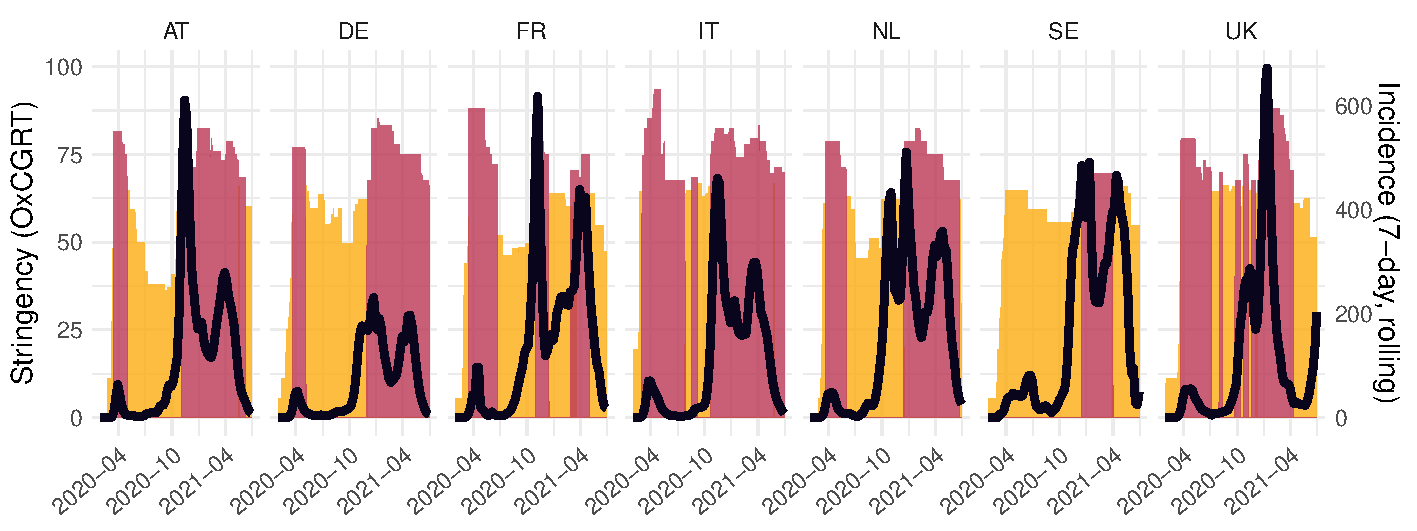
\includegraphics{plots/p_realw_20240226.pdf}

}

\caption{COVID-19 Incidences and Policy Stringency Over Time by Country}

\end{figure}

In Figure 1, the stringency level for each country throughout the
observed time frame is plotted as a colored histogram and the 7-day
incidence rate as a line. The red bars mark phases when containment
policies were stricter than the overall median, the yellow bars indicate
below-median phases. Expecting that policies affect comments with some
delay, this study lagged the stringency variable by 14 days. The lag was
chosen based on its somewhat stronger correlation with populism (.07),
compared to other lags. Time was operationalized by a variable counting
the days since the World Health Organization declared the pandemic on
March 11, 2020, and by a dummy indicating if the post was published
during the \emph{first wave} of COVID-19.

\hypertarget{control-variables}{%
\subsubsection{Control Variables}\label{control-variables}}

Controls include the 14-day lagged \emph{incidence rate} (i.e., the
weekly rolling number of new infections per 100.000 inhabitants in a
country-day format, retrieved from the OxCRT). Additional controls are
the number of \emph{comments} per post, \emph{download age} (i.e., days
passed between post and download), and the logged number of Facebook
\emph{fans}. Table 4 presents the summary statistics. Continuous
independent variables were standardized and centered on the population
mean before being included in the models.

\hypertarget{model-specifications}{%
\subsubsection{Model Specifications}\label{model-specifications}}

Linear regression was used for hypothesis testing, as the dependent
variable is continuous. Accounting for the nested structure of the data,
with posts nested in pages, and pages nested in countries, multilevel
models were fitted (Gelman and Hill 2007). The small number of
country-level clusters and the non-randomness of the sample create
problems for frequentist inference (Chan and Rauchfleisch 2023).

Accounting for both, the models were fitted in a Bayesian framework,
using the \emph{brms} package (Bürkner et al. 2022). Media type could be
considered an additional level but was included as a fixed effect, as it
has only three categories. Model 1 accounts for random intercepts for
countries and pages. Model 2 drops four variables to avoid
over-parameterization and adds two interaction terms. Model 3 fits
random slopes for COVID-19, stringency, and their interaction across all
countries. The models were fitted using non-informative priors, and
3,000 iterations of three chains that converged.

\newpage
{
\begin{spacing}{.9}
\fontsize{9}{10}\selectfont 
\begin{longtable}[]{@{}
  >{\raggedright\arraybackslash}p{.35\linewidth}
  >{\raggedleft\arraybackslash}p{.11\linewidth}
  >{\raggedleft\arraybackslash}p{.11\linewidth}
  >{\raggedleft\arraybackslash}p{.11\linewidth}
  >{\raggedleft\arraybackslash}p{.11\linewidth}@{}}
\caption{Summary Statistics} \\
\toprule\noalign{}
\textbf{Variables} & \textbf{Min.} & \textbf{Max.} & \textbf{Mean / n} & \textbf{SD / \%} \\
\midrule\noalign{}
\endhead
\endlastfoot
\emph{Dependent variable} & & & &  \\
\quad Populism\textsuperscript{a} & -7.4 &  4.4 &   0.0 &   (1.0) \\
\emph{Explanatory variables} & & & & \\ 
\quad COVID-19 & 0 &    1 & 24,378 & (37\%) \\
\quad Restrictions & 0 & 1 & 11,204 &   (17\%) \\
\quad Government & 0 & 1 & 8,681 & (13\%) \\
\quad Experts & 0 & 1 & 7,271 & (11\%) \\
\quad Moderation & 0 & 1 & 3,184 & (4.9\%) \\
\quad Days since outbreak\textsuperscript{b,c} & -38.7 &    476.0   & 244.9 &   (148.6) \\
\quad First wave\textsuperscript{d} &   0 & 1 & 17,177 &    (26\%) \\
\quad Stringency \tiny(14-day lag)\small\textsuperscript{b} &   0 & 93.5 &  61.3 &  (21.3) \\
\emph{Controls} & & & &  \\
\quad Incidence rate \tiny(14-day lag)\small\textsuperscript{b,e} & 0 & 631.6 & 114.9   & (117.3)\\
\quad Download age\textsuperscript{b} & 0 & 416.2 & 127.0   & (120.1) \\
\quad Comments count\textsuperscript{b} &   0 & 23,829.0 &  197.2 & (544.5) \\
\quad Fan count \tiny(log)\small\textsuperscript{b} &   12.2 &  17.8 &  14.0 &  (1.3) \\
\emph{Media type} & & & & \\                
\qquad Quality & & & 22,694 &   (35\%) \\
\qquad Tabloid & & &    22,122 &    (34\%) \\
\qquad Public broadcaster & & & 20,442 & (31\%) \\
\emph{Country} & & & & \\               
\qquad Austria (AT) & & & 12,345 & (19\%) \\
\qquad Germany (DE) & & & 10,066 & (15\%) \\
\qquad France (FR) & & & 8,818 &    (13\%) \\
\qquad Italy (IT) & & & 8,547   & (13\%) \\
\qquad Netherlands (NL) & & & 9,913 & (15\%) \\
\qquad Sweden (SE) & & & 9,123  & (14\%) \\
\qquad United Kingdom (UK) & & & 6,446  & (9.9\%) \\
\midrule\noalign{}
\quad \textbf{N} & & & \textbf{65,258} & \\
\midrule\noalign{}
\multicolumn{5}{@{}m{\textwidth}@{}}{\tiny{\emph{Notes:} (a) Post-level mean, standardized and centered on country mean; (b) Standardized and centered at population mean in models; (c) WHO declared pandemic on March 11, 2021; (d) Published before 6 July, 2020 (incidences low); (e) New infections per 100,000 inhabitants in 7 days, rolling.}}   \\
\end{longtable}
\end{spacing}
}

\hypertarget{results}{%
\subsection{Results}\label{results}}

Table 5 reports the results from the linear multilevel Bayesian
regression models with the mean populism score per post as the dependent
variable. H1 proposed that posts mentioning the \emph{government} are
associated with higher levels of populism in the comments section. The
parameter .49 for \emph{government} in Model 1 marks the median of the
estimated posterior distribution. All else being equal, the aggregated
populism score is estimated to increase by .49 standard deviations when
a post mentions the government. The credible interval (CI) indicates
that 95\% of the posterior draws for that parameter lie between 0.47 and
0.51. Figure 2 plots the posterior distributions of the variables in
Model 1, showing that \emph{government} has the strongest positive
effect. As its 95\% highest density interval (HDI), here identical with
the CI, excludes zero, the null hypothesis is rejected and H1 supported.
Similarly, in support of H2, mentioning \emph{experts} has a large
(.13), positive effect, with a CI excluding zero {[}.11--.15{]}.

RQ1 asked for the impact of \emph{moderating comments} on user-generated
populism. Model 1 shows that this relationship is negative (-.13,
{[}-.16 -- -.09{]}). Comments sections including comments from the media
outlet itself were less populist. Somewhat surprisingly, \emph{media
type tabloid} is negatively associated with populism (RQ2). Compared to
the reference category, \emph{quality media}, comments sections on
Facebook pages of tabloids received -.37 {[}-.55 -- -.17{]} less
populist comments. Public broadcasters did not receive significantly
more populist comments than the quality press, as the CI {[}-.09--.29{]}
includes zero.

The COVID-19 specific predictors in Model 1 show that posts mentioning
\emph{COVID-19} were associated with .17 {[}.15 -- .19{]} higher levels
of populism in comments than other posts. This was the second-largest
positive effect in the model, as shown in Figure 1. Posts explicitly
mentioning \emph{restrictions}, a sub-category of COVID-19 posts, were
associated with .06 {[}.04--.09{]} more populist comments. These
findings support H3 and H4.

The effects of time were in accordance with expectations (H6 and H7).
With each \emph{day since the outbreak}, the level of populism in
comments increased by .02 {[}.00--.04{]}. The negative effect of the
predictor \emph{first wave} was pronounced, indicating that comments
sections below posts published during the first wave of COVID-19 were
.17 {[}-.20 -- -.14{]} SD less populist than comments sections of later
posts.

The main effect of \emph{stringency} in COVID-19 policies was positive
but very small (.03). Its credible interval {[}.02-.04{]} in Model 1
excludes zero but barely so. In Model 2 and Model 3, the CI includes
zero. These models explore the conditions under which stringency had a
positive impact more closely.

\newpage
{
\begin{spacing}{.9}
\fontsize{9}{10}\selectfont 
\begin{longtable}[]{@{}
  >{\raggedright\arraybackslash}p{0.21\linewidth}
  >{\centering\arraybackslash}p{0.06\linewidth}
  >{\centering\arraybackslash}p{0.125\linewidth}
  >{\centering\arraybackslash}p{0.06\linewidth}
  >{\centering\arraybackslash}p{0.125\linewidth}
  >{\centering\arraybackslash}p{0.06\linewidth}
  >{\centering\arraybackslash}p{0.125\linewidth}@{}}
\caption{Results of the Bayesian Multilevel Linear Regression Models} \\
\toprule\noalign{}
\begin{minipage}[b]{\linewidth}\raggedright
\end{minipage} & 
\multicolumn{2}{p{0.21\linewidth}}{\centering
\textbf{Model 1}
} &
\multicolumn{2}{p{0.21\linewidth}}{\centering
\textbf{Model 2}
} &
\multicolumn{2}{p{0.21\linewidth}}{\centering
\textbf{Model 3}
} \\
\emph{Predictors} & 
\multicolumn{1}{c}{\emph{Est.}} &
\multicolumn{1}{c}{\emph{CI (95\%)}} &
\multicolumn{1}{c}{\emph{Est.}} &
\multicolumn{1}{c}{\emph{CI (95\%)}} &
\multicolumn{1}{c}{\emph{Est.}} &
\multicolumn{1}{c}{\emph{CI (95\%)}} \\
\midrule\noalign{}
\endhead
%\bottomrule\noalign{}
\endlastfoot
Intercept & -.01 & -.15 -- .13 & -.01 & -.13 -- .13 & -.00 & -.14 -- .13 \\
COVID-19 \tiny (mentioned) & .17 & .15 -- .19 & .20 & .19 -- .22 & .20 & .12 -- .28 \\
Restrictions \tiny (mentioned) & .06 & .04 -- .09 & & & & \\
Government \tiny (mentioned) & .49 & .47 -- .51 & .49 & .47 -- .51 & .49 & .47 -- .51 \\
Experts \tiny (mentioned) & .13 & .11 -- .15 & .13 & .11 -- .15 & .13 & .11 -- .15 \\
Moderation & -.13 & -.16 -- -.09 & -.13 & -.16 -- -.09 & -.12 & -.15 -- -.08 \\
Media type \tiny (tabloid) & -.37 & -.55 -- -.17 & -.37 & -.55 -- -.19 & -.37 & -.55 -- -.18 \\
Media type \newline \tiny (pub. broadcaster) & .10 & -.09 -- .29 & .09 & -.09 -- .27 & .09 & -.10 -- .27 \\
Stringency \tiny (lagged) & .03 & .02 -- .04 & -.00 & -.01 -- .01 & -.00 & -.07 -- .07 \\
Days since outbreak & .02 & .00 -- .04 & .03 & .02 -- .04 & .02 & .01 -- .03 \\
First wave & -.17 & -.20 -- -.14 & -.18 & -.21 -- -.15 & -.19 & -.22 -- -.16 \\
Comments count & .16 & .15 -- .16 & .16 & .15 -- .17 & .16 & .15 -- .17 \\
Download age & -.01 & -.03 -- .00 & & & & \\
Fan count \tiny (log) & -.01 & -.09 -- .07 & & & & \\
Incidence \tiny(lagged) & -.00 & -.01 -- .01 & & & & \\
COVID-19 * \newline Stringency & & & .07 & .06 -- .09 & .05 & -.02 -- .12 \\
\\
\emph{Random Effects} & & & & & & \\
\tiny $\sigma^{2}$ & \multicolumn{1}{l}{\tiny .84} & & \multicolumn{1}{l}{\tiny .84} & & \multicolumn{1}{l}{\tiny .83} & \\
\tiny $\tau_{00}$ & \multicolumn{2}{l}{\tiny .03\textsubscript{Page}}  & \multicolumn{2}{l}{\tiny .03\textsubscript{Page}}  & \multicolumn{2}{l}{\tiny .03\textsubscript{Page}} \\
\tiny & \tiny .00\textsubscript{Country} & & \tiny .00\textsubscript{Country} & & \tiny .01\textsubscript{Country} & \\
\tiny $\tau_{11}$ & & & & & \multicolumn{2}{l}{\tiny .01\textsubscript{Country:COVID-19}}\\
\tiny & & & & & \multicolumn{2}{l}{\tiny .01 \textsubscript{Country:Stringency}} \\
\tiny & & & & & \multicolumn{2}{l}{\tiny .01 \textsubscript{Country:COVID-19:Strg.}}  \\
\tiny ICC & \multicolumn{1}{l}{\tiny.04} & & \multicolumn{1}{l}{\tiny.03} & & \multicolumn{1}{l}{\tiny.06} & \\
\tiny Levels & 7\tiny\textsubscript{Country} & & 7\tiny\textsubscript{Country} & & 7\tiny\textsubscript{Country} & \\
\multicolumn{1}{c}{\centering } & 21\tiny\textsubscript{Page} & & 21\tiny\textsubscript{Page} & & 21\tiny\textsubscript{Page} & \\
\midrule\noalign{}
Bayes R\textsuperscript{2} &  \multicolumn{1}{l}{.162} & .158 -- .167 &  \multicolumn{1}{l}{.164} & .159 -- .168 &  \multicolumn{1}{l}{.168} & .163 -- .172 \\
N & 65,258 & & 65,258 & & 65,258 & \\
\midrule\noalign{}
\multicolumn{7}{l}{\tiny{\emph{Notes:} Priors: intercept (normal 0, 10), b (normal 0, 10), $\sigma$ (Cauchy 0, .5).}} \\
\multicolumn{7}{l}{\tiny{Bayes R\textsuperscript{2} estimated on 2,000 draws.}} \\ 
\end{longtable}
\end{spacing} 
}

\begin{figure}

{\centering 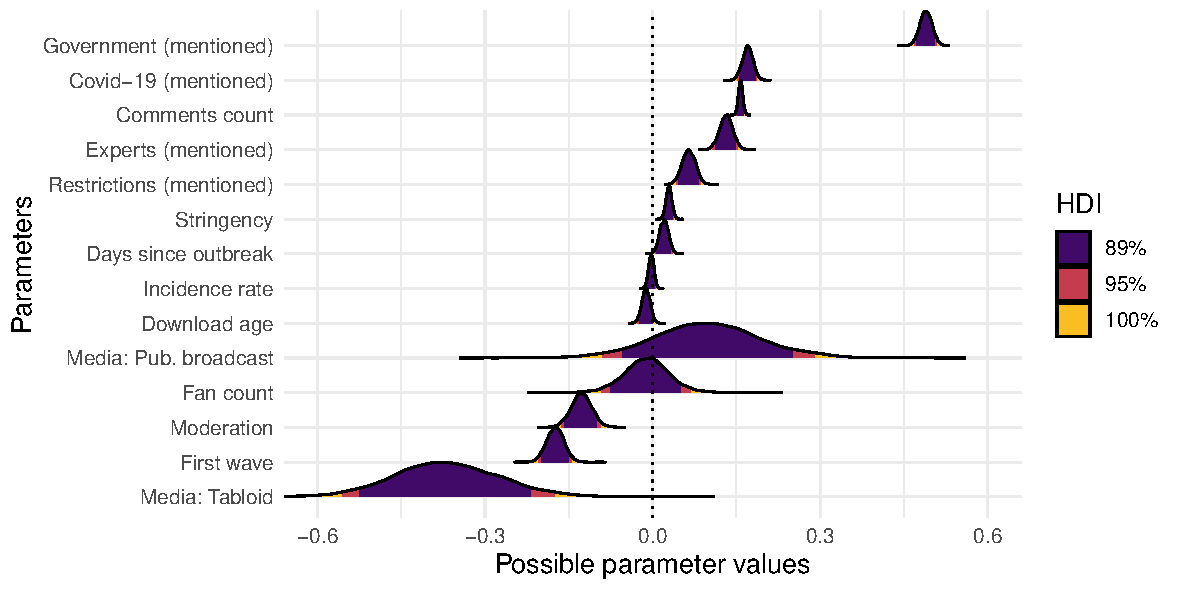
\includegraphics{plots/hdi_m3b_20240226.pdf}

}

\caption{Highest-Density-Intervals (HDI) of Predictors in Model 1}

\end{figure}

Before moving on, the random effects of Model 1 should be noted. The
within-group variance (sig\textsuperscript{2}=.84) is large, while the
between-group variance for pages is small (tau\textsubscript{00}=.03),
and zero for countries, which is also reflected in the small intra-class
correlation coefficient (ICC) of .04. Zero variance between countries is
unsurprising, as the dependent variable was centered on country mean.
Fitting random intercepts for the level country would not have been
necessary. I kept this grouping variable, as Model 3 introduces random
slopes on this level.

Model 2 functions as intermediate step and adds the interaction term
\emph{COVID-19*Stringency.} To reduce model complexity, the
insignificant control variables \emph{fan count, incidence}, and
\emph{download age} were dropped, as well as the variable
\emph{restrictions,} which is not independent of \emph{COVID-19}. The
positive and significant coefficient for the interaction term
\emph{COVID-19*Stringency} suggests an interplay between mentioning
COVID-19 and the restrictiveness of policies, as expected in H5.
However, the main effect of stringency diminished.

To explore this pattern from a comparative perspective across countries,
and to answer RQ3, Model 3 estimates random slopes (i.e., varying
effects) for \emph{COVID-19, stringency,} and their interaction
\emph{COVID-19*Stringency} by \emph{country}. The random slopes variance
(tau\textsubscript{11}=.01) of Model 3 is larger than zero. While the CI
of both \emph{stringency} and the term \emph{COVID-19*Stringency} now
include zero, a substantive effect of stringency can be found for
specific countries. Figure 3 plots the distribution of the posterior
predictions of populism on the y-axis, conditional on the level of
stringency (x-axis and color) for each country. For this prediction,
mentioning \emph{COVID-19} was set to ``true,'' \emph{media type} was
set to ``quality'' and all other variables were held at mean,
respectively zero. Uncertainty from the page level was accounted for.

Figure 3 visualizes three things: The colored half-eye plots show the
distribution of the predicted level of populism when stringency is at
its minimum (yellow) and its maximum (purple) per country. The black dot
marks the median, the thick bar the 80\% CI, and the thin bar the 89\%
CI of this distribution. The layering thin lines illustrate the
estimated relationship on 300 draws.

The plot shows that \emph{stringency} had a positive effect in Austria,
Germany, and the Netherlands, when \emph{COVID-19} was mentioned. For
these countries, the thick 80\% CI bars for the stringency at minimum
and at maximum conditions do not overlap; the draws illustrate the
positive estimated relationship. However, for Austria and Netherlands,
this relationship is only credible when accepting an 80\% CI. For
Germany, this finding also holds on a 95\% CI. In the other countries,
the relationship is diffuse, insignificant, and even slightly reversed.
This illustrates why the effect is cancelled out on the population
level. This pattern also emerges when fitting separate models per
country (Appendix E). Overall, the evidence for H5 is mixed. Of the
control variables, only \emph{comments count} had a significant positive
effect on the level of populism. The Bayes-R\textsuperscript{2}
indicates that the models explain 16.2-16.8\% of the variance.

\begin{figure}

{\centering 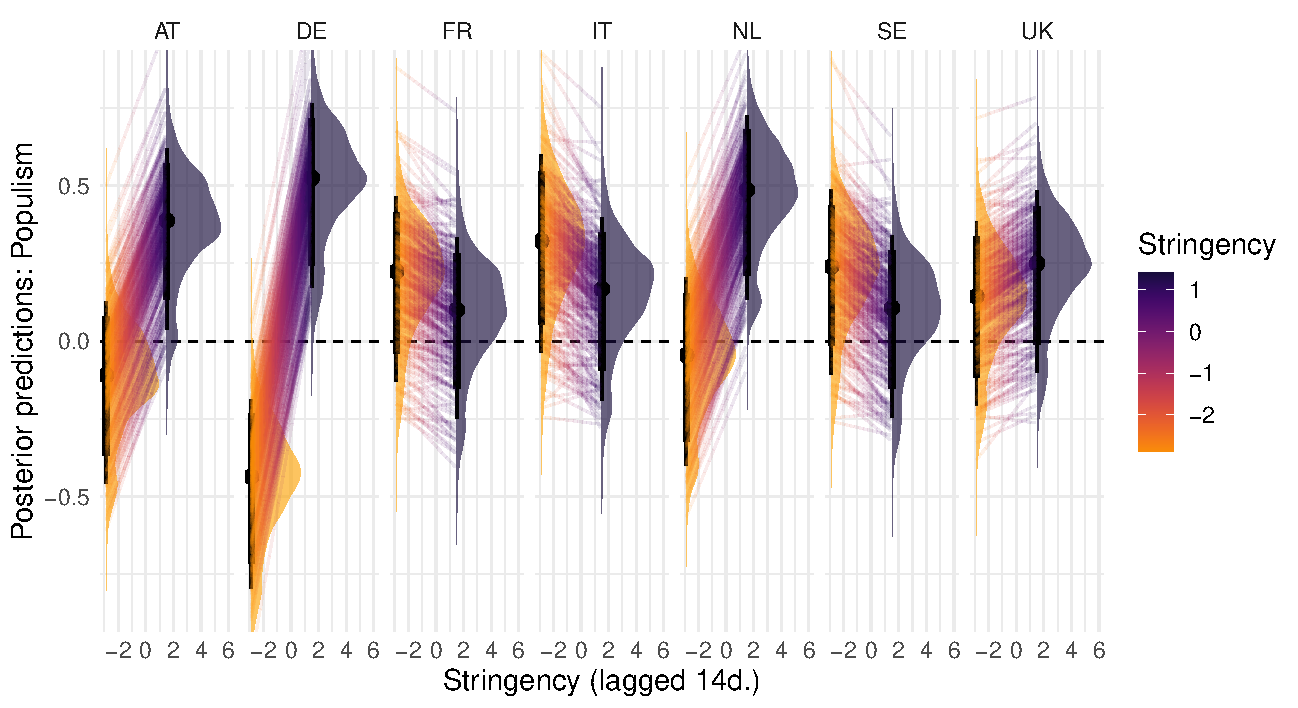
\includegraphics{plots/plot_M11_strgXcov_byctry_LINES_300draws_20240226.pdf}

}

\caption{Posterior Predictions of Populism by Stringency Across
Countries -- Model 3}

\end{figure}

\hypertarget{discussion-and-conclusions}{%
\subsection{Discussion and
Conclusions}\label{discussion-and-conclusions}}

This study analyzed how the COVID-19 crisis and media-related factors
shaped the levels of populism in user comments on news media Facebook
pages in seven European countries. It revealed several noteworthy
findings. First, Facebook posts mentioning \emph{COVID-19} and
\emph{restrictive containment policies} were associated with higher
levels of populism in comments, compared to other posts. These findings
provide circumstantial evidence for the argument that media coverage on
COVID-19 motivated some users to express populist ideas by triggering
reactance and activating populist attitudes. COVID-19 was an issue that
mobilized populist protests not only on the streets (Brubaker 2021) but
also online. Populism in comments also increased considerably after the
first wave of COVID-19, adding behavioral evidence to the finding of a
``pandemic fatigue'' which has fueled populist attitudes over time
(Jørgensen et al. 2022). The findings largely confirm previous findings
for Germany and Austria (Thiele 2022a) and align with psychological
research showing that novel messages spark less reactance (Rosenberg and
Siegel 2018).

Second, this study found that the \emph{stringency} of COVID-19 policies
had a varying impact on populism in comments across countries. At the
population level, the effect was mainly cancelled out by diverging
effects across countries. A comparative analysis found a limited
positive effect of containment policy stringency for Austria, Germany,
and the Netherlands. In these countries, stricter COVID-19 containment
policies were echoed by more populism in comments, when the post
mentioned COVID-19. The question is why this relationship was not
observed in all countries. In Sweden, the laissez-faire containment
policies may have prevented populist discontent (Gordon, Grafton, and
Steinshamn 2021). In Italy, the shock of the devastating first wave
might have increased acceptance of stringent policies. Finding ad-hoc
explanations for France and the United Kingdom is difficult. Future
research should investigate these differences by taking governmental
communication strategies and strategies of grassroots mobilization
(Neumayer, Pfaff, and Plümper 2023) into account.

Third, mentioning elite representatives was found to have triggered
populism. Mentioning the government had the strongest effect on populism
in comments, replicating a previous finding (Thiele 2022a). Different
from my previous findings (Thiele 2022a), posts mentioning experts were
here found to be associated with more populism. These different findings
can be driven by differences in the sample as well as by different
operationalizations. This finding also shows that science-related
populism (Mede and Schäfer 2020) is an important aspect of
user-generated populism. Overall, the study shows that the level of
populism in comments is highly responsive to the content and context of
posts. This finding contributes to the plausibility of the argument that
populist comments are expressions of populist attitudes (Blassnig,
Engesser, et al. 2019), that are activated by message characteristics
(Krämer 2014) and context (Hawkins, Rovira Kaltwasser, and Andreadis
2020). Additional research is needed, however, to investigate the
presumed mechanisms directly.

Fourth, my findings did not corroborate the existence of a
``complicity'' between the tabloid press and populism (Mazzoleni 2008,
50) on the level of user comments. Tabloid outlets received the lowest
levels of populism in comments. However, this does not necessarily imply
that readers of tabloids are less populist (Schulz 2019). Populist users
may deliberately visit the pages of quality press and public service
broadcasters to express discontent because they regard these to be part
of the establishment (Engesser et al. 2017). Fifth, this study found
that comments authored by the media page itself lowered the levels of
populism. This finding is indirect support for the effectiveness of
visible moderation (Gibson 2019).

This study has implications beyond the context of COVID-19. Contributing
to a more comprehensive understanding of citizen-generated populist
communication, the study identified factors influencing populism in
comments that may hold in other contexts---mentioning elites,
moderation, and media type. Moreover, the lessons learned during
COVID-19 can be projected onto other contexts concerning science-related
populism (Mede and Schäfer 2020). The debates surrounding climate change
resemble the COVID-19 crisis in crucial aspects: Climate change
communication tries to convince people to comply with restrictive
policies that are necessary to avert a global threat (Nabi, Gustafson,
and Jensen 2018). This aim is similarly challenged by citizens'
reactance (Ma, Dixon, and Hmielowski 2019) and populist online behavior
(Yan, Schroeder, and Stier 2022). Drawing on the findings here, one
could expect that climate change coverage similarly attracts populist
comments. Building on the country-specific relation between policy
stringency and populism found here, policymakers could be cautiously
optimistic that governance can shape the level of populist discontent
expressed online. More research is needed, however, to substantiate
these claims and investigate the role of governmental communication more
thoroughly. Finally, newsrooms worried about the harmful effects of
populist user comments can feel encouraged that visibly moderating their
comments sections can have a beneficial impact.

Methodologically, this study contributed to the field of computational
communication science by demonstrating the usefulness of the DDR
technique (Garten et al. 2018) for capturing ideological content. The
strengths of this method are that it provides a theory-driven, and
interpretable measurement (Garten et al. 2018, 351), as the core of the
measured concept can be gleaned from keywords. At the same time, it is
more flexible than conventional dictionaries by leveraging the potential
of word embeddings. The advantage of word embeddings over transformers
and large language models is that training on a custom corpus can be
performed on a local machine and is computationally relatively
inexpensive. This study has also contributed to the growing field of
multilingual computational text analysis (Licht and Lind 2023) by
demonstrating the usefulness -- and limitations -- of a full-text
machine translation approach. Future research can build on these
experiences.

\hypertarget{limitations}{%
\subsection{Limitations}\label{limitations}}

This study has limitations. First, validating the populism score
revealed imperfect measurement equivalence and potential measurement
error differential to language. Such error can cause bias in regressions
(TeBlunthuis, Hase, and Chan 2023) and is of particular concern for the
cross-country comparison. TeBlunthuis et al. (2023) recently introduced
a correction for misclassification error in regression analyses. Here,
implementing this correction was not possible as the manually annotated
data only provides a binary indicator of populism, not its ``true''
continuous value. The problem was approached here by centering the
populism score on the country mean, assuming that focusing on
within-country variance improves comparability. As this builds on strong
assumptions, the results of the country comparison must be taken with a
grain of salt. Another problem is that measurement error inflicted by
translation could not be discerned from error induced by
country-specific discourse. Future computational text analyses should
annotate validation data on the same scale as the automated measurement
to enable error correction. Continuous measurements could be validated
against aggregated scores of multiple annotators, to circumvent the
challenge of producing reliable continuous annotations (Grimmer and
Stewart 2013, 275). Second, machine translation is one strategy for
aligning the input of multilingual computational text analyses (Licht
and Lind 2023) that is not free of problems. In addition to the
imperfect measurement equivalence observed discussed above, commercial
translation APIs pose challenges for replicating findings, as they
change, are non-transparent, and are expensive. Local implementations or
multilingual embeddings are alternatives that should be considered.
Finally, this study did not test individual-level mechanisms directly,
as the anonymized digital trace data does not provide observations on
this level. Future research is encouraged to test the claims of this
study using experimental research designs.

\hypertarget{additional-materials}{%
\subsection{Additional materials}\label{additional-materials}}

The dictvectoR package (Thiele 2022b) is available on GitHub.
Replication code and data is provided here: https://osf.io/d4qng/

\hypertarget{declaration-of-conflicting-interests}{%
\subsection{Declaration of Conflicting
Interests}\label{declaration-of-conflicting-interests}}

The author declares no potential conflicts of interest.

\hypertarget{acknowledgements}{%
\subsection{Acknowledgements}\label{acknowledgements}}

This research was supported by the Kaiserschild Foundation, the Austrian
Federal Ministry of Education, Science and Research through an OeAD
Marietta Blau‐Scholarship {[}MPC‐2021‐02005{]}, and the German Federal
Ministry of Education and Research under grant number 16DII135.

\hypertarget{references}{%
\subsection{References}\label{references}}

\hypertarget{refs}{}
\begin{CSLReferences}{1}{0}
\leavevmode\vadjust pre{\hypertarget{ref-aslanidis2018MeasuringPopulist}{}}%
Aslanidis, Paris. 2018. {``Measuring Populist Discourse with Semantic
Text Analysis: An Application on Grassroots Populist Mobilization.''}
\emph{Quality \& Quantity} 52 (3): 1241--63.
\url{https://doi.org/10.1007/s11135-017-0517-4}.

\leavevmode\vadjust pre{\hypertarget{ref-benesty2019Fastrtext}{}}%
Benesty, Michaël. 2019. {``Fastrtext 0.3.4.''}
\url{https://github.com/pommedeterresautee/fastrtext}.

\leavevmode\vadjust pre{\hypertarget{ref-benoit2018QuantedaPackage}{}}%
Benoit, Kenneth, Kohei Watanabe, Haiyan Wang, Paul Nulty, Adam Obeng,
Stefan Müller, and Akitaka Matsuo. 2018. {``Quanteda. {An R} Package for
the Quantitative Analysis of Textual Data.''} \emph{Journal of Open
Source Software} 3 (30): 774. \url{https://doi.org/10.21105/joss.00774}.

\leavevmode\vadjust pre{\hypertarget{ref-blassnig2019HittingNerve}{}}%
Blassnig, Sina, Sven Engesser, Nicole Ernst, and Frank Esser. 2019.
{``Hitting a Nerve: {Populist} News Articles Lead to More Frequent and
More Populist Reader Comments.''} \emph{Political Communication} 36 (4):
629--51. \url{https://doi.org/10.1080/10584609.2019.1637980}.

\leavevmode\vadjust pre{\hypertarget{ref-blassnig2016CodebookPopulist}{}}%
Blassnig, Sina, Sven Engesser, and Frank Esser. 2016. \emph{Codebook:
{Populist} Online Communication in {Europe}: {Self-presentation}, Media
Representation, and Audience Reconstruction of Political Actors}.
{Z{ü}rich}: {Courtesy by the Authors}.

\leavevmode\vadjust pre{\hypertarget{ref-blassnig2019PopulismOnline}{}}%
Blassnig, Sina, Nicole Ernst, Florin Büchel, Sven Engesser, and Frank
Esser. 2019. {``Populism in {Online Election Coverage}.''}
\emph{Journalism Studies} 20 (8): 1110--29.
\url{https://doi.org/10.1080/1461670X.2018.1487802}.

\leavevmode\vadjust pre{\hypertarget{ref-bojanowski2017EnrichingWord}{}}%
Bojanowski, Piotr, Edouard Grave, Armand Joulin, and Tomas Mikolov.
2017. {``Enriching Word Vectors with Subword Information.''}
\emph{arXiv:1607.04606 {[}Cs{]}}, June.
\url{http://arxiv.org/abs/1607.04606}.

\leavevmode\vadjust pre{\hypertarget{ref-bos2014PopulistRhetoric}{}}%
Bos, Linda, and Kees Brants. 2014. {``Populist Rhetoric in Politics and
Media: {A} Longitudinal Study of the {Netherlands}.''} \emph{European
Journal of Communication} 29 (6): 703--19.
\url{https://doi.org/10.1177/0267323114545709}.

\leavevmode\vadjust pre{\hypertarget{ref-brehm1966TheoryPsychological}{}}%
Brehm, Jack Williams. 1966. \emph{A Theory of Psychological Reactance}.
{New York}: {Academic Press}.

\leavevmode\vadjust pre{\hypertarget{ref-brehm1981PsychologicalReactance}{}}%
Brehm, Sharon S., and Jack Williams Brehm. 1981. \emph{Psychological
Reactance: A Theory of Freedom and Control}. {New York}: {Academic
Press}.

\leavevmode\vadjust pre{\hypertarget{ref-brubaker2021ParadoxesPopulism}{}}%
Brubaker, Rogers. 2021. {``Paradoxes of Populism During the Pandemic.''}
\emph{Thesis Eleven} 164 (1): 73--87.
\url{https://doi.org/10.1177/0725513620970804}.

\leavevmode\vadjust pre{\hypertarget{ref-burkner2022BrmsBayesian}{}}%
Bürkner, Paul-Christian, Jonah Gabry, Sebastian Weber, Andrew Johnson,
Martin Modrak, Hamada S. Badr, Frank Weber, Mattan S. Ben-Shachar,
Hayden Rabel, and Simon C. Mills. 2022. {``Brms: {Bayesian Regression
Models} Using '{Stan}'.''}
\url{https://CRAN.R-project.org/package=brms}.

\leavevmode\vadjust pre{\hypertarget{ref-canovan1999TrustPeople}{}}%
Canovan, Margaret. 1999. {``Trust the People! {Populism} and the Two
Faces of Democracy.''} \emph{Political Studies} 47 (1): 2--16.
\url{https://doi.org/10.1111/1467-9248.00184}.

\leavevmode\vadjust pre{\hypertarget{ref-chan2023BayesianMultilevel}{}}%
Chan, Chung-Hong, and Adrian Rauchfleisch. 2023. {``Bayesian {Multilevel
Modeling} and {Its Application} in {Comparative Journalism Studies}.''}
\emph{International Journal of Communication} 17 (0): 3700--3721.
\url{https://ijoc.org/index.php/ijoc/article/view/19570}.

\leavevmode\vadjust pre{\hypertarget{ref-coe2014OnlineUncivil}{}}%
Coe, Kevin, Kate Kenski, and Stephen A. Rains. 2014. {``Online and
Uncivil? {Patterns} and Determinants of Incivility in Newspaper Website
Comments.''} \emph{Journal of Communication} 64 (4): 658--79.
\url{https://doi.org/10.1111/jcom.12104}.

\leavevmode\vadjust pre{\hypertarget{ref-dahlberg2011ReconstructingDigital}{}}%
Dahlberg, Lincoln. 2011. {``Re-Constructing Digital Democracy: {An}
Outline of Four {`Positions'}.''} \emph{New Media \& Society} 13 (6):
855--72. \url{https://doi.org/10.1177/1461444810389569}.

\leavevmode\vadjust pre{\hypertarget{ref-devreese2018PopulismExpression}{}}%
de Vreese, Claes H., Frank Esser, Toril Aalberg, Carsten Reinemann, and
James Stanyer. 2018. {``Populism as an Expression of Political
Communication Content and Style: {A} New Perspective.''} \emph{The
International Journal of Press/Politics} 23 (4): 423--38.
\url{https://doi.org/10.1177/1940161218790035}.

\leavevmode\vadjust pre{\hypertarget{ref-dillard2005NatureReactance}{}}%
Dillard, James Price, and Lijiang Shen. 2005. {``On the Nature of
Reactance and Its Role in Persuasive Health Communication.''}
\emph{Communication Monographs} 72 (2): 144--68.
\url{https://doi.org/10.1080/03637750500111815}.

\leavevmode\vadjust pre{\hypertarget{ref-dillard2023PersuasiveMessages}{}}%
Dillard, James Price, Xi Tian, Shannon M. Cruz, Rachel A. Smith, and
Lijiang Shen. 2023. {``Persuasive {Messages}, {Social Norms}, and
{Reactance}: {A Study} of {Masking Behavior} During a {COVID-19 Campus
Health Campaign}.''} \emph{Health Communication} 38 (7): 1338--48.
\url{https://doi.org/10.1080/10410236.2021.2007579}.

\leavevmode\vadjust pre{\hypertarget{ref-engesser2017PopulismSocial}{}}%
Engesser, Sven, Nicole Ernst, Frank Esser, and Florin Büchel. 2017.
{``Populism and Social Media: How Politicians Spread a Fragmented
Ideology.''} \emph{Information, Communication \& Society} 20 (8):
1109--26. \url{https://doi.org/10.1080/1369118X.2016.1207697}.

\leavevmode\vadjust pre{\hypertarget{ref-ernst2019PopulistsPrefer}{}}%
Ernst, Nicole, Sina Blassnig, Sven Engesser, Florin Büchel, and Frank
Esser. 2019. {``Populists Prefer Social Media over Talk Shows: {An}
Analysis of Populist Messages and Stylistic Elements Across Six
Countries.''} \emph{Social Media + Society} 5 (1): 1--14.
\url{https://doi.org/10.1177/2056305118823358}.

\leavevmode\vadjust pre{\hypertarget{ref-esau2017DesignMatters}{}}%
Esau, Katharina, Dennis Friess, and Christiane Eilders. 2017. {``Design
Matters! {An} Empirical Analysis of Online Deliberation on Different
News Platforms.''} \emph{Policy \& Internet} 9 (3): 321--42.
\url{https://doi.org/10.1002/poi3.154}.

\leavevmode\vadjust pre{\hypertarget{ref-flew2021GlobalTrust}{}}%
Flew, Terry. 2021. {``The {Global Trust Deficit Disorder}: {A
Communications Perspective} on {Trust} in the {Time} of {Global
Pandemics}.''} \emph{Journal of Communication} 71 (2): 163--86.
\url{https://doi.org/10.1093/joc/jqab006}.

\leavevmode\vadjust pre{\hypertarget{ref-galpin2019ParticipatoryPopulism}{}}%
Galpin, Charlotte, and Hans-Jörg Trenz. 2019. {``Participatory Populism:
{Online} Discussion Forums on Mainstream News Sites During the 2014
{European Parliament} Election.''} \emph{Journalism Practice} 13 (7):
781--98. \url{https://doi.org/10.1080/17512786.2019.1577164}.

\leavevmode\vadjust pre{\hypertarget{ref-garten2018DictionariesDistributions}{}}%
Garten, Justin, Joe Hoover, Kate M. Johnson, Reihane Boghrati, Carol
Iskiwitch, and Morteza Dehghani. 2018. {``Dictionaries and
Distributions: {Combining} Expert Knowledge and Large Scale Textual Data
Content Analysis.''} \emph{Behavior Research Methods} 50 (1): 344--61.
\url{https://doi.org/10.3758/s13428-017-0875-9}.

\leavevmode\vadjust pre{\hypertarget{ref-gelman2007DataAnalysis}{}}%
Gelman, Andrew, and Jennifer Hill. 2007. \emph{Data Analysis Using
Regression and Multilevel/Hierarchical Models}. Analytical Methods for
Social Research. {Cambridge ; New York}: {Cambridge University Press}.

\leavevmode\vadjust pre{\hypertarget{ref-gerbaudo2018SocialMedia}{}}%
Gerbaudo, Paolo. 2018. {``Social Media and Populism: An Elective
Affinity?''} \emph{Media, Culture \& Society} 40 (5): 745--53.
\url{https://doi.org/10.1177/0163443718772192}.

\leavevmode\vadjust pre{\hypertarget{ref-gibson2019FreeSpeech}{}}%
Gibson, Anna. 2019. {``Free {Speech} and {Safe Spaces}: {How Moderation
Policies Shape Online Discussion Spaces}.''} \emph{Social Media +
Society} 5 (1). \url{https://doi.org/10.1177/2056305119832588}.

\leavevmode\vadjust pre{\hypertarget{ref-gordon2021CrosscountryEffects}{}}%
Gordon, Daniel V., R. Quentin Grafton, and Stein Ivar Steinshamn. 2021.
{``Cross-Country Effects and Policy Responses to {COVID-19} in 2020:
{The Nordic} Countries.''} \emph{Economic Analysis and Policy} 71
(September): 198--210. \url{https://doi.org/10.1016/j.eap.2021.04.015}.

\leavevmode\vadjust pre{\hypertarget{ref-grimmer2013TextData}{}}%
Grimmer, Justin, and Brandon M. Stewart. 2013. {``Text as Data: {The}
Promise and Pitfalls of Automatic Content Analysis Methods for Political
Texts.''} \emph{Political Analysis} 21 (3): 267--97.
\url{https://doi.org/10.1093/pan/mps028}.

\leavevmode\vadjust pre{\hypertarget{ref-grundl2022PopulistIdeas}{}}%
Gründl, Johann. 2022. {``Populist Ideas on Social Media: {A}
Dictionary-Based Measurement of Populist Communication.''} \emph{New
Media \& Society} 24 (6): 1481--99.
\url{https://doi.org/10.1177/1461444820976970}.

\leavevmode\vadjust pre{\hypertarget{ref-hajek2021ParadoxesReactance}{}}%
Hajek, Katharina V., and Michael Häfner. 2021. {``Paradoxes of
{Reactance During} the {COVID-19 Pandemic}: {A Social-psychological
Perspective}.''} \emph{Javnost - The Public} 28 (3): 290--305.
\url{https://doi.org/10.1080/13183222.2021.1969619}.

\leavevmode\vadjust pre{\hypertarget{ref-hale2020OxfordCOVID19}{}}%
Hale, Thomas, Noam Angrist, Emily Cameron-Blake, Laura Hallas, Beatriz
Kira, Saptarshi Majumdar, Anna Petherick, Toby Phillips, and Helen
Tatlow. 2020. {``Oxford {COVID-19} Government Response Tracker.''}
{Blavatnik School of Government}.
\url{https://www.bsg.ox.ac.uk/research/research-projects/coronavirus-government-response-tracker}.

\leavevmode\vadjust pre{\hypertarget{ref-hallin2004ComparingMedia}{}}%
Hallin, Daniel C., and Paolo Mancini. 2004. \emph{Comparing {Media
Systems}: {Three Models} of {Media} and {Politics}}. {Cambridge/New York
a.o.}: {Cambridge University Press}.

\leavevmode\vadjust pre{\hypertarget{ref-hameleers2019PopulismOnline}{}}%
Hameleers, Michael. 2019. {``The Populism of Online Communities:
{Constructing} the Boundary Between {`Blameless'} People and
{`Culpable'} Others.''} \emph{Communication, Culture and Critique} 12
(1): 147--65. \url{https://doi.org/10.1093/ccc/tcz009}.

\leavevmode\vadjust pre{\hypertarget{ref-hameleers2021EffectsPopulist}{}}%
Hameleers, Michael, Desirée Schmuck, Anne Schulz, Dominique Stefanie
Wirz, Jörg Matthes, Linda Bos, Nicoleta Corbu, and Ioannis Andreadis.
2021. {``The {Effects} of {Populist Identity Framing} on {Populist
Attitudes Across Europe}: {Evidence From} a 15-{Country Comparative
Experiment}.''} \emph{International Journal of Public Opinion Research}
33 (3): 491--510. \url{https://doi.org/10.1093/ijpor/edaa018}.

\leavevmode\vadjust pre{\hypertarget{ref-hawkins2018IntroductionIdeational}{}}%
Hawkins, Kirk A., and Cristóbal Rovira Kaltwasser. 2018.
{``Introduction. {The} Ideational Approach.''} In \emph{The {Ideational
Approach} to {Populism}. {Concept}, {Theory}, and {Analysis}}, edited by
Kirk A. Hawkins, Ryan E. Carlin, Levente Littvay, and Cristóbal Rovira
Kaltwasser, 1--24. {Routledge}.

\leavevmode\vadjust pre{\hypertarget{ref-hawkins2020ActivationPopulist}{}}%
Hawkins, Kirk A., Cristobal Rovira Kaltwasser, and Ioannis Andreadis.
2020. {``The {Activation} of {Populist Attitudes}.''} \emph{Government
and Opposition} 55 (2): 283--307.
\url{https://doi.org/10.1017/gov.2018.23}.

\leavevmode\vadjust pre{\hypertarget{ref-jagers2007PopulismPolitical}{}}%
Jagers, Jan, and Stefaan Walgrave. 2007. {``Populism as Political
Communication Style: {An} Empirical Study of Political Parties'
Discourse in {Belgium}.''} \emph{European Journal of Political Research}
46 (3): 319--45. \url{https://doi.org/10.1111/j.1475-6765.2006.00690.x}.

\leavevmode\vadjust pre{\hypertarget{ref-jorgensen2022PandemicFatigue}{}}%
Jørgensen, Frederik, Alexander Bor, Magnus Storm Rasmussen, Marie Fly
Lindholt, and Michael Bang Petersen. 2022. {``Pandemic Fatigue~Fueled
Political Discontent During the {COVID-19} Pandemic.''}
\emph{Proceedings of the National Academy of Sciences} 119 (48):
e2201266119. \url{https://doi.org/10.1073/pnas.2201266119}.

\leavevmode\vadjust pre{\hypertarget{ref-jost2020PopulismFuels}{}}%
Jost, Pablo, Marcus Maurer, and Joerg Hassler. 2020. {``Populism Fuels
Love and Anger: {The} Impact of Message Features on Users' Reactions on
{Facebook}.''} \emph{International Journal of Communication} 14 (0):
2081--2102.
\url{https://www.ijoc.org/index.php/ijoc/article/view/13400}.

\leavevmode\vadjust pre{\hypertarget{ref-junger2020FacepagerApplication}{}}%
Jünger, Jakob, and Till Keyling. 2020. {``Facepager. {An} Application
for Automated Data Retrieval on the Web.''}
\url{https://github.com/strohne/Facepager/}.

\leavevmode\vadjust pre{\hypertarget{ref-klinger2015EmergenceNetwork}{}}%
Klinger, Ulrike, and Jakob Svensson. 2015. {``The Emergence of Network
Media Logic in Political Communication: {A} Theoretical Approach.''}
\emph{New Media \& Society} 17 (8): 1241--57.
\url{https://doi.org/10.1177/1461444814522952}.

\leavevmode\vadjust pre{\hypertarget{ref-koch2013HelpfulHarmful}{}}%
Koch, Thomas, and Thomas Zerback. 2013. {``Helpful or Harmful? {How}
Frequent Repetition Affects Perceived Statement Credibility.''}
\emph{Journal of Communication} 63 (6): 993--1010.
\url{https://doi.org/10.1111/jcom.12063}.

\leavevmode\vadjust pre{\hypertarget{ref-kramer2014MediaPopulism}{}}%
Krämer, Benjamin. 2014. {``Media Populism: {A} Conceptual Clarification
and Some Theses on Its Effects.''} \emph{Communication Theory} 24 (1):
42--60. \url{https://doi.org/10.1111/comt.12029}.

\leavevmode\vadjust pre{\hypertarget{ref-kriesi2023ProtestUnlikely}{}}%
Kriesi, Hanspeter, and Ioana-Elena Oana. 2023. {``Protest in Unlikely
Times: Dynamics of Collective Mobilization in {Europe} During the
{COVID-19} Crisis.''} \emph{Journal of European Public Policy} 30 (4):
740--65. \url{https://doi.org/10.1080/13501763.2022.2140819}.

\leavevmode\vadjust pre{\hypertarget{ref-licht2023GoingCrosslingual}{}}%
Licht, Hauke, and Fabienne Lind. 2023. {``Going Cross-Lingual: {A} Guide
to Multilingual Text Analysis.''} \emph{Computational Communication
Research} 5 (2): 1--31. \url{https://doi.org/10.5117/CCR2023.2.2.LICH}.

\leavevmode\vadjust pre{\hypertarget{ref-ma2019PsychologicalReactance}{}}%
Ma, Yanni, Graham Dixon, and Jay D. Hmielowski. 2019. {``Psychological
{Reactance From Reading Basic Facts} on {Climate Change}: {The Role} of
{Prior Views} and {Political Identification}.''} \emph{Environmental
Communication} 13 (1): 71--86.
\url{https://doi.org/10.1080/17524032.2018.1548369}.

\leavevmode\vadjust pre{\hypertarget{ref-marcos-marne2023WhatWe}{}}%
Marcos-Marne, Hugo, Homero Gil de Zúñiga, and Porismita Borah. 2023.
{``What Do We (Not) Know about Demand-Side Populism? {A} Systematic
Literature Review on Populist Attitudes.''} \emph{European Political
Science} 22 (3): 293--307.
\url{https://doi.org/10.1057/s41304-022-00397-3}.

\leavevmode\vadjust pre{\hypertarget{ref-matthes2018SpiralSilence}{}}%
Matthes, Jörg, Johannes Knoll, and Christian von Sikorski. 2018. {``The
{`{Spiral} of {Silence}'} {Revisited}: {A Meta-Analysis} on the
{Relationship Between Perceptions} of {Opinion Support} and {Political
Opinion Expression}.''} \emph{Communication Research} 45 (1): 3--33.
\url{https://doi.org/10.1177/0093650217745429}.

\leavevmode\vadjust pre{\hypertarget{ref-mazzoleni2008PopulismMedia}{}}%
Mazzoleni, Gianpietro. 2008. {``Populism and the Media.''} In
\emph{Twenty-First Century Populism. {The} Spectre of {Western European}
Democracy}, edited by Daniele Albertazzi and Duncan McDonnell, 49--64.
{Basingstoke/New York}: {Palgrave MacMillan}.

\leavevmode\vadjust pre{\hypertarget{ref-mede2020SciencerelatedPopulism}{}}%
Mede, Niels G., and Mike S. Schäfer. 2020. {``Science-Related Populism:
{Conceptualizing} Populist Demands Toward Science.''} \emph{Public
Understanding of Science} 29 (5): 473--91.
\url{https://doi.org/10.1177/0963662520924259}.

\leavevmode\vadjust pre{\hypertarget{ref-mikolov2013EfficientEstimation}{}}%
Mikolov, Tomas, Kai Chen, Greg Corrado, and Jeffrey Dean. 2013.
{``Efficient {Estimation} of {Word Representations} in {Vector
Space}.''} \emph{arXiv:1301.3781 {[}Cs{]}}, September.
\url{http://arxiv.org/abs/1301.3781}.

\leavevmode\vadjust pre{\hypertarget{ref-mudde2004PopulistZeitgeist}{}}%
Mudde, Cas. 2004. {``The Populist Zeitgeist.''} \emph{Government and
Opposition} 39 (4): 541--63.
\url{https://doi.org/10.1111/j.1477-7053.2004.00135.x}.

\leavevmode\vadjust pre{\hypertarget{ref-mudde2007PopulistRadical}{}}%
---------. 2007. \emph{Populist Radical Right Parties in {Europe}}.
{Cambridge}: {Cambridge University Press}.

\leavevmode\vadjust pre{\hypertarget{ref-nabi2018FramingClimate}{}}%
Nabi, Robin L., Abel Gustafson, and Risa Jensen. 2018. {``Framing
{Climate Change}: {Exploring} the {Role} of {Emotion} in {Generating
Advocacy Behavior}.''} \emph{Science Communication} 40 (4): 442--68.
\url{https://doi.org/10.1177/1075547018776019}.

\leavevmode\vadjust pre{\hypertarget{ref-neumayer2023ProtestCovid19}{}}%
Neumayer, Eric, Katharina Gabriela Pfaff, and Thomas Plümper. 2023.
{``Protest Against {Covid-19} Containment Policies in {European}
Countries.''} \emph{Journal of Peace Research}, February.
\url{https://doi.org/10.1177/00223433221135335}.

\leavevmode\vadjust pre{\hypertarget{ref-newman2022ReutersInstitute}{}}%
Newman, Nic, Richard Fletcher, Craig T. Robertson, Kirsten Eddy, and
Rasmus Kleis Nielsen. 2022. \emph{Reuters Institute Digital News Report
2022}. {Reuters Institute for the Study of Journalism}.
\url{https://reutersinstitute.politics.ox.ac.uk/digital-news-report/2022}.

\leavevmode\vadjust pre{\hypertarget{ref-organ1974SocialExchange}{}}%
Organ, Dennis W. 1974. {``Social Exchange and Psychological Reactance in
a Simulated Superior-Subordinate Relationship.''} \emph{Organizational
Behavior and Human Performance} 12 (1): 132--42.
\url{https://doi.org/10.1016/0030-5073(74)90042-7}.

\leavevmode\vadjust pre{\hypertarget{ref-quandt2018DarkParticipation}{}}%
Quandt, Thorsten. 2018. {``Dark Participation.''} \emph{Media and
Communication} 6 (4): 36--48.
\url{https://doi.org/10.17645/mac.v6i4.1519}.

\leavevmode\vadjust pre{\hypertarget{ref-rauh2018ValidatingSentiment}{}}%
Rauh, Christian. 2018. {``Validating a Sentiment Dictionary for {German}
Political Language---a Workbench Note.''} \emph{Journal of Information
Technology \& Politics} 15 (4): 319--43.
\url{https://doi.org/10.1080/19331681.2018.1485608}.

\leavevmode\vadjust pre{\hypertarget{ref-rico2017EmotionalUnderpinnings}{}}%
Rico, Guillem, Marc Guinjoan, and Eva Anduiza. 2017. {``The {Emotional
Underpinnings} of {Populism}: {How Anger} and {Fear Affect Populist
Attitudes}.''} \emph{Swiss Political Science Review} 23 (4): 444--61.
\url{https://doi.org/10.1111/spsr.12261}.

\leavevmode\vadjust pre{\hypertarget{ref-righetti2022OnsetInfodemic}{}}%
Righetti, Nicola, Luca Rossi, and Giada Marino. 2022. {``At the Onset of
an Infodemic: {Geographic} and Disciplinary Boundaries in Researching
Problematic {COVID-19} Information.''} \emph{First Monday}, July.
\url{https://doi.org/10.5210/fm.v27i7.12557}.

\leavevmode\vadjust pre{\hypertarget{ref-rooduijn2019StateField}{}}%
Rooduijn, Matthijs. 2019. {``State of the Field: {How} to Study Populism
and Adjacent Topics? {A} Plea for Both More and Less Focus.''}
\emph{European Journal of Political Research} 58 (1): 362--72.
\url{https://doi.org/10.1111/1475-6765.12314}.

\leavevmode\vadjust pre{\hypertarget{ref-rosenberg201850YearReview}{}}%
Rosenberg, Benjamin, and Jason Siegel. 2018. {``A 50-{Year Review} of
{Psychological Reactance Theory}: {Do Not Read This Article}.''}
\emph{Motivation Science} 4 (December): 281--300.
\url{https://doi.org/10.1037/mot0000091}.

\leavevmode\vadjust pre{\hypertarget{ref-schraff2021PoliticalTrust}{}}%
Schraff, Dominik. 2021. {``Political Trust During the {Covid-19}
Pandemic: {Rally} Around the Flag or Lockdown Effects?''} \emph{European
Journal of Political Research} 60 (4): 1007--17.
\url{https://doi.org/10.1111/1475-6765.12425}.

\leavevmode\vadjust pre{\hypertarget{ref-schulz2019WherePopulist}{}}%
Schulz, Anne. 2019. {``Where Populist Citizens Get the News: {An}
Investigation of News Audience Polarization Along Populist Attitudes in
11 Countries.''} \emph{Communication Monographs} 86 (1): 88--111.
\url{https://doi.org/10.1080/03637751.2018.1508876}.

\leavevmode\vadjust pre{\hypertarget{ref-sherrick2018EffectExplicit}{}}%
Sherrick, Brett, and Jennifer Hoewe. 2018. {``The Effect of Explicit
Online Comment Moderation on Three Spiral of Silence Outcomes.''}
\emph{New Media \& Society} 20 (2): 453--74.
\url{https://doi.org/10.1177/1461444816662477}.

\leavevmode\vadjust pre{\hypertarget{ref-stecula2021HowPopulism}{}}%
Stecula, Dominik A., and Mark Pickup. 2021. {``How Populism and
Conservative Media Fuel Conspiracy Beliefs about {COVID-19} and What It
Means for {COVID-19} Behaviors.''} \emph{Research \& Politics} 8 (1).
\url{https://doi.org/10.1177/2053168021993979}.

\leavevmode\vadjust pre{\hypertarget{ref-sun2023HowMisinformation}{}}%
Sun, Yanqing, and Fangcao Lu. 2023. {``How {Misinformation} and
{Rebuttals} in {Online Comments Affect People}'s {Intention} to {Receive
COVID-19 Vaccines}: {The Roles} of {Psychological Reactance} and
{Misperceptions}.''} \emph{Journalism \& Mass Communication Quarterly}
100 (1): 145--71. \url{https://doi.org/10.1177/10776990221084606}.

\leavevmode\vadjust pre{\hypertarget{ref-teblunthuis2023MisclassificationAutomated}{}}%
TeBlunthuis, Nathan, Valerie Hase, and Chung-Hong Chan. 2023.
{``Misclassification in {Automated Content Analysis Causes Bias} in
{Regression}. {Can We Fix It}? {Yes We Can}!''} {arXiv}.
\url{https://doi.org/10.48550/arXiv.2307.06483}.

\leavevmode\vadjust pre{\hypertarget{ref-thiele2022PandemicPopulism}{}}%
Thiele, Daniel. 2022a. {``Pandemic Populism? {How Covid-19} Triggered
Populist {Facebook} User Comments in {Germany} and {Austria}.''}
\emph{Politics and Governance} 10 (1): 185--96.
\url{https://doi.org/10.17645/pag.v10i1.4712}.

\leavevmode\vadjust pre{\hypertarget{ref-thiele2022ThieledDictvectoR}{}}%
---------. 2022b. {``Thieled/{dictvectoR}.''}
\url{https://doi.org/10.5281/zenodo.7079600}.

\leavevmode\vadjust pre{\hypertarget{ref-thiele2022HowRightWing}{}}%
Thiele, Daniel, and Tjaša Turnšek. 2022. {``How {Right-Wing Populist
Comments Affect Online Deliberation} on {News Media Facebook Pages}.''}
\emph{Media and Communication} 10 (4): 141--54.
\url{https://doi.org/10.17645/mac.v10i4.5690}.

\leavevmode\vadjust pre{\hypertarget{ref-vries2018NoLonger}{}}%
Vries, Erik de, Martijn Schoonvelde, and Gijs Schumacher. 2018. {``No
{Longer Lost} in {Translation}: {Evidence} That {Google Translate Works}
for {Comparative Bag-of-Words Text Applications}.''} \emph{Political
Analysis} 26 (4): 417--30. \url{https://doi.org/10.1017/pan.2018.26}.

\leavevmode\vadjust pre{\hypertarget{ref-waisbord2018WhyPopulism}{}}%
Waisbord, Silvio. 2018. {``Why Populism Is Troubling for Democratic
Communication.''} \emph{Communication, Culture and Critique} 11 (1):
21--34. \url{https://doi.org/10.1093/ccc/tcx005}.

\leavevmode\vadjust pre{\hypertarget{ref-wettstein2019WhatDrives}{}}%
Wettstein, Martin, Frank Esser, Florin Büchel, Christian Schemer,
Dominique S. Wirz, Anne Schulz, Nicole Ernst, Sven Engesser, Philipp
Müller, and Werner Wirth. 2019. {``What {Drives Populist Styles}?
{Analyzing Immigration} and {Labor Market News} in 11 {Countries}.''}
\emph{Journalism \& Mass Communication Quarterly} 96 (2): 516--36.
\url{https://doi.org/10.1177/1077699018805408}.

\leavevmode\vadjust pre{\hypertarget{ref-wintterlin2020HowCope}{}}%
Wintterlin, Florian, Tim Schatto-Eckrodt, Lena Frischlich, Svenja
Boberg, and Thorsten Quandt. 2020. {``How to {Cope} with {Dark
Participation}: {Moderation Practices} in {German Newsrooms}.''}
\emph{Digital Journalism} 8 (7): 904--24.
\url{https://doi.org/10.1080/21670811.2020.1797519}.

\leavevmode\vadjust pre{\hypertarget{ref-witte1992PuttingFear}{}}%
Witte, Kim. 1992. {``Putting the Fear Back into Fear Appeals: {The}
Extended Parallel Process Model.''} \emph{Communication Monographs} 59
(4): 329--49. \url{https://doi.org/10.1080/03637759209376276}.

\leavevmode\vadjust pre{\hypertarget{ref-wondreys2022VictimsPandemic}{}}%
Wondreys, Jakub, and Cas Mudde. 2022. {``Victims of the {Pandemic}?
{European Far-Right Parties} and {COVID-19}.''} \emph{Nationalities
Papers} 50 (1): 86--103. \url{https://doi.org/10.1017/nps.2020.93}.

\leavevmode\vadjust pre{\hypertarget{ref-yan2022ThereLink}{}}%
Yan, Pu, Ralph Schroeder, and Sebastian Stier. 2022. {``Is There a Link
Between Climate Change Scepticism and Populism? {An} Analysis of Web
Tracking and Survey Data from {Europe} and the {US}.''}
\emph{Information, Communication \& Society} 25 (10): 1400--1439.
\url{https://doi.org/10.1080/1369118X.2020.1864005}.

\end{CSLReferences}

\newpage
\appendix
\renewcommand{\thefigure}{A\arabic{figure}}
\renewcommand{\thetable}{A\arabic{table}}
\setcounter{figure}{0}
\setcounter{table}{0}

\hypertarget{appendix-a}{%
\subsection{Appendix A}\label{appendix-a}}

\hypertarget{coding-instructions}{%
\subsubsection{Coding Instructions}\label{coding-instructions}}

Here, I document an abridged version of the coding instructions for
annotating the validation data. Comments were coded along the binary
variables \emph{people-centrism} and \emph{anti-elitism,} covering key
messages of populist communication. The coding instructions for populism
align with the codebook developed by Blassnig et al. (2016; 2019) and
have been used in part in my previous studies (Thiele 2022a; Thiele and
Turnšek 2022).

At the post level, coders assigned binary values for the presence of
references to the \emph{government}, \emph{experts}, \emph{COVID-19},
\emph{COVID-19 policies}, and \emph{easing of COVID-19 policies.} The
last two variables were used to construct the variable references to
\emph{COVID-19 policy restrictions}.

Holistic grading was employed for coding comments and posts, i.e.~the
complete post or comment was considered in assigning codes. Coders were
presented with general coding instructions, adopted from Blassnig et al.
(2016, 1): ``Only code explicit statements. Implications, hints, and
context knowledge must not be coded. If in doubt, don't code it. If you
have to ask yourself whether a statement is explicit enough to code it,
it is not. {[}\ldots{]} Hypothetical statements are coded. Statements
that are future-oriented or in subjunctive mood are coded as normal
statements. Hypothetical does not mean implicit.'' The general
instructions additionally clarified that the categories are not mutually
exclusive, addressed the handling of missing values, and explained the
filter variables.

\hypertarget{post-level-variables}{%
\subsubsection{Post-Level Variables}\label{post-level-variables}}

{
\begin{spacing}{1}
\fontsize{8}{9}\selectfont 
\begin{longtable}[]{@{}
  >{\raggedright\arraybackslash}p{.14\linewidth}
  >{\raggedright\arraybackslash}p{.62\linewidth}
  >{\raggedright\arraybackslash}p{.13\linewidth}@{}}
\caption{Coding Instructions for Posts} \\
\toprule\noalign{}
\textbf{Construct} & \textbf{Instructions} & \textbf{Codes} \\
\midrule\noalign{}
\endhead
\endlastfoot
\emph{Topic:} COVID-19 mentioned & 
\emph{Question:} \newline Does the post mention the topic of COVID-19? \newline \newline
\emph{Instructions:} \newline Please code “1” if the coded text refers in some form to the COVID-19 virus, or any aspect of the COVID-19 pandemic, including any governmental, societal, or scientific response to, or consequence of, the COVID-19 crisis. 
& 
0: not present \newline
1: present
\\
\emph{Subtopic:} \newline
COVID-19 policies
&
\emph{FILTER:  If “covid” = “0”, this category is  “0”. \newline If “covid” = “1”, please code:} \newline \newline 
\emph{Question:} \newline Does the post mention any authorities’ measure responding to the COVID-19 crisis? \newline \newline
\emph{Definitions:} \newline
“Authorities” here mean all levels of government, whether national, regional, local, or supra-national, all public service agencies, all public health advisory boards or councils (e.g., the RKI in Germany, the RIVM in Netherlands, the Folkhälsomyndigheten in Sweden etc.), and local institutions such as schools or hospitals. \newline
& 
0: not present \newline
1: present
\\
&
"COVID-19 measures" include, but are not limited to, measures directed at public health (e.g., social distancing, masks, quarantine, hygienic rules), including testing for COVID-19 or vaccinations; restrictive measures (e.g., closing of schools, restaurants, lockdowns, measures limiting social contacts); contact tracing; travel restrictions and specific border policies; policies that ease COVID-19 restrictions; policies that react on economic or social challenges related to the COVID-19 crisis. References to the general COVID-crisis management of authorities are also considerd as ‘COVID-19 policies’ here. \newline
& 
\\
&
\emph{Instructions:} \newline Please code “1” if the coded text refers in some form to any measure of authorities that is a response to the COVID-19 crisis – whether directed at public health or other aspects of the crisis. 
& 
\\
\emph{Subtopic:}
Easing COVID-19 policies
&
\emph{FILTER:  If “covid policy” = “0”, this category is  “0”. \newline 
If “covid policy” = “1”, please code:} \newline \newline 
\emph{Question:} \newline Does the post mention any easing of restrictive COVID-19 policies, or policies that offer economic support? \newline \newline
\emph{Instructions:} \newline Please code “1” if the coded text refers in some form to easing restrictive measures (e.g., mentions of lifting lockdowns, lifting obligatory mask wearing, lifting travel bans, lifting restrictions to enter public events); or measures intended to cushion economic or social hardships induced by the COVID-19 crisis (e.g., emergency funds, helplines). \newline
& 
0: not present \newline
1: present
\\ 
\emph{Actors:}
Government
&
\emph{Question:} \newline Does the post mention the current national government of the country in question or the European Commission? \newline \newline
\emph{Definitions:} \newline
The “government” here exclusively refers to the incumbent (at the time of the post) head of government (e.g., Prime Minister, Chancellor, in France: including the President), the ministers of his or her cabinet, the government as a whole, and the European Commission. 
\newline
& 
0: not present \newline
1: present
\\ 
& 
Mentioning the head of state (only exception: “the President” in France); parliamentarians who are not part of the cabinet; public advisory boards; regional or local governing bodies; foreign governments; or former governments do not count as ‘the government’ here. \newline
&
\\
&
\emph{Instructions:} \newline
Please code “1” if the coded text refers to the head of the current national government of the respective country at the time of the post – referred to by either his or her name or office; any minister of the (federal) government of the respective country at that time – referred to by either his or her name or office; the government as a whole; the head or any member of the European Commission at that time; the European Commission as a whole. 
\newline \newline 
\emph{Note: A list of names, official titles and incumbents was provided to the coders.}
&
\\
\emph{Actors:}
Experts
&
\emph{Question:} \newline Does the post mention experts? \newline \newline
\emph{Definitions:} \newline An “expert” here is understood as someone who has acquired profound knowledge in a specific field through academic education or research. We consider experts from any field of knowledge, whether public health related or not. Persons who have acquired profound experience through practice but without academic education are not considered experts here (e.g., general healthcare professionals). References to the output or field of study of those experts, as well as references to public research institutions is considered as mentioning experts. Explicit references to “experts” do count. 
& 
0: not present \newline
1: present
\\ 
&
References to private research institutions (e.g., BioNTech, Pfizer) is not sufficient to be counted as mentioning “experts” here. If the post refers explicitly to the researchers active in, or research conducted at, those institutions this counts as mentioning experts. \newline
&
\\
&
\emph{Instructions:} \newline
Please code “1” if the coded text refers to anyone explicitly as “expert”, or “specialist”; to any researchers – either in general terms (e.g., “researcher”, “scientist”), by indicating their area of expertise (e.g., “virologist”, “psychologist”, “virology”, “psychology”), or by indicating their academic profession (e.g., “professor XY”); research in general (e.g., “research”, “a study”, “science”); any public, academic research institution (e.g., “university XY”, “institute XY”); other public health experts with an academic backgroud (e.g. physicians or doctors).  
Please note that mentioning general healthcare professionals of hospitals does not count as reference to experts here.
&
\\
\midrule\noalign{}
\end{longtable}
\end{spacing}
}

\hypertarget{comment-level-variables}{%
\subsubsection{Comment-Level Variables}\label{comment-level-variables}}

{
\begin{spacing}{1}
\fontsize{8}{9}\selectfont 
\begin{longtable}[]{@{}
  >{\raggedright\arraybackslash}p{.14\linewidth}
  >{\raggedright\arraybackslash}p{.62\linewidth}
  >{\raggedright\arraybackslash}p{.13\linewidth}@{}}
\caption{Coding Instructions for Comments} \\
\toprule\noalign{}
\textbf{Construct} & \textbf{Instructions} & \textbf{Codes} \\
\midrule\noalign{}
\endhead
\endlastfoot
People-centrism & 
\emph{Question:} \newline Does the comment invoke the people or demand sovereignty for the people? (Aslanidis, 2018, 1255) \newline \newline
\emph{Definitions:} \newline People-centrism is one core dimension of populist communication. It is defined here as an ideological discourse that invokes ‘the people’ (Aslanidis 2018, 1255). It values ‘the people’ as something positive or worth protecting, constructs it as an in-group, i.e., as a group to which the author of the text belongs to, and/or suggests that ‘the people’ are the “rightful political sovereign within a given polity” (Aslanidis 2018, 1255).
& 
0: not present \newline
1: present
\\
& ‘The people’ are defined as the “overwhelming majority” (Aslanidis 2018, 1255) of the “population of a country” or polity that is assumed to “share a common origin or culture” (Blassnig et al. 2016, 14). “The people may be regarded as nation, ethnos, demos, class, or strata” (Blassnig et al. 2016, 14). It is essential that the commenter regards himself or herself as part of the people and values the people. The people may be addressed directly (“the people”, “the Austrian population”), “as a metaphor (‘man on the street’, ‘the common man’), or as a subgroup that is regarded as representing” (Blassnig et al. 2016, 14) the overwhelming majority (‘the hardworking people’, ‘voters’, ‘we taxpayers’). & 
\\
&
\emph{Instructions:} \newline
Please code “1”, if the coded text refers to ‘the people’ in one of the ways described above and is characterized by at least one of the following aspects: \newline
&
\\
&
\begin{itemize}
\item The people are attributed with virtues and positive traits. For example, the people may be described as good, honest, hard-working, modest, moral, credible, intelligent, competent, consistent, considerate, benevolent, or similar (Blassnig et al., 2016 , 17). (e.g., “every normal citizen knows about this madness”)
\end{itemize}
&
\\
&
\begin{itemize}
\item The people are seen as responsible for positive developments, events, or situations (Blassnig et al. 2016, 17). (e.g., “I am glad to be a tiny part of this. A lot of work and sweat has built this country and made it what it is now.”)
\end{itemize}
&
\\
&
\begin{itemize}\item The people are described as a homogeneous group: The “people is seen as sharing a common understanding of the world, common feelings [...], common opinions [...], or a common will [...].  (e.g., ‘The voters want immigration controlled, they declared that loud and clear.’)” (Blassnig et al. 2016, 18).
\end{itemize}
&
\\
&
\begin{itemize}\item The people are constructed as a collective of victims, that suffers from elite actions, or external threats, or needs to be protected (Hameleers, 2019). (e.g.: “Who is protecting us????”)
\end{itemize}
&
\\
&
\begin{itemize}\item The comment demands to listen to the people’s will, or addresses the people to wake up, or to stand up for their will (Blassnig et al. 2016, 20) (e.g., “let’s unite and take the streets! together we can make a difference!”)
\end{itemize}
&
\\
&
\begin{itemize}\item The comment criticizes institutions or elites for not reflecting the people’s will, for deceiving or silencing the vast majority. (e.g.: “The people will not be deceived any longer by this clown.”)
\end{itemize}
&
\\
Anti-elitism & 
\emph{Question:} \newline Does the comment discredit or blame the elite or suggest that the elite is detached from the people? (Blassnig et al. 2016, 18–19) \newline \newline
\emph{Definitions:} \newline Anti-elitism is the second core dimension of populist communication. It is defined as “references against a slim minority of unaccountable power holders [that allegedly engage] [...] in the misappropriation of popular sovereignty” (Aslanidis 2018, 1255). It constructs ‘the elite’ as the antagonist of ‘the people’, which illegitimately rules and deceives the latter (Mudde 2004, 543).
& 
0: not present \newline
1: present
\\
& 
‘The elite’ is defined as minority groups of power holders within a society that are (assumed to be) powerful and influential because of its “political power, wealth, or privilege” (Blassnig et al. 2016, 14). Not the factual power is decisive, but the assumption of such power in the coded text. Elites “can be allocated to the areas of politics, administration, economy, law, media, science, and culture” (Blassnig et al. 2016, 14). “The elite may either be addressed in general terms [(e.g., ‘those above’, ‘politicians’, ‘the rich’, ‘the media’)] or specific members [or institutional representatives] of the elite may be addressed by name” (Blassnig et al. 2016, 14) or nickname (e.g., “Wall Street”, “Brussels”, “Soros”).
& 
\\
&
\emph{Instructions:} \newline
Please code “1”, if the coded text refers to ‘the elite’ in some of the ways described above and is characterized by at least one of the following aspects: \newline
&
\\
&
\begin{itemize}
\item Elites are discredited or denounced: “Negative personality traits, mistakes, and unlawful or immoral behavior of the elites are stressed. The elites [...] are portrayed as corrupt, evil, incapable, malevolent, [mendacious], criminal, lazy, stupid, undemocratic [or in any other similar negative way]. The elites or its representatives are denied of morality, charisma, credibility, intelligence, competence, consistency etc.” (Blassnig et al. 2016, 18) (e.g., “It is minister Mikl Leitner who, apart from incompetence, only attracts attention with embarrassing statements.”; “Down with this sell-out government!”) \newline
\emph{Caution:} If a text criticizes elites in a balanced way, without suggesting a fundamental or moral degeneracy of the elite or the established system it is not considered anti-elitist. 
\end{itemize}
\\
&
\begin{itemize}\item Elites are blamed for fundamentally negative developments or situations: elites are held responsible for undesirable situations that are depicted as serious harm for the society (Blassnig et al. 2016, 18). (e.g., “Our politicians have managed to make Austria an unsafe country. The politicians who are responsible should be locked up”)
\end{itemize}
&
\\
&
\begin{itemize}\item Elites are depicted as detached from the people, unaccountable to the people’s will, or manipulating the people: The elite is described as “not being close to the people, not knowing the people and their needs, not speaking for the people, [...] not listening to the people,” (Blassnig et al. 2016, 19) not representing the people, betraying or deceiving the people, lying to the people, manipulating the public opinion, or as being distanced from the people in any other way (Blassnig et al. 2016, 19–20). (e.g., “when will our so-called representatives of the people finally open their eyes”; “The politicians do not listen to us”)
\end{itemize}
&
\\
&
\begin{itemize}\item Elites are denied sovereignty. “The speaker argues in favor of granting less power to the” or some elites (Blassnig et al. 2016, 21). (e.g., “I hope that the EU breaks apart so that Austria can finally close the borders!)
\end{itemize}
&
\\
\midrule\noalign{}
\end{longtable}
\end{spacing}
}

\newpage
\renewcommand{\thefigure}{B\arabic{figure}}
\renewcommand{\thetable}{B\arabic{table}}
\setcounter{figure}{0}
\setcounter{table}{0}

\hypertarget{appendix-b}{%
\subsection{Appendix B}\label{appendix-b}}

\hypertarget{text-cleaning-and-preprocessing}{%
\subsubsection{Text Cleaning and
Preprocessing}\label{text-cleaning-and-preprocessing}}

Text was cleaned and preprocessed for the tasks: (a) translation, (b)
training the \emph{fastText} model, (c) measurement development, (d)
application of the post-level dictionaries, and (e) application of the
DDR measurements. For most tasks, text was lowercased, punctuation,
hyperlinks, and stop-words were removed, numbers, emojis and emoticons
were replaced by words. Stop-words were defined following the German
\emph{nltk} list, with the exception of the following words that were
considered to function as in- and out-group marker in populist discourse
or convey other important meaning: \emph{alle*, diese*, die, das,
einige*, euer*, eur*, uns*, keine*, mein*, nicht*, solche*, sie, sich,
nur, wieder, selbst, manche*, seine*, wir}. Emojis were manually
assigned by the author to four broad emotion categories joy, anger,
fear, and other. Table B1 documents all replaced emojis and other
special characters.

Text cleaning was applied as consistently as possible in all steps of
the analysis, with some exceptions. These exceptions are: (a) For
translation, text was not lowercased, punctuation only simplified,
emojis replaced after translation, and text truncated to 540 characters;
(b) For training the \emph{fastText} model, no stop-words were removed,
text was tokenized into sentences and shuffled, duplicates and comments
with less than 5 words were removed; (c) For applying the case-sensitive
dictionary for government representatives on post level, text was not
lowercased to capture names correctly.

{
\begin{spacing}{.9}
\fontsize{7}{8}\selectfont 
\begin{longtable}[]{@{}
  >{\raggedright\arraybackslash}p{(\columnwidth - 0\tabcolsep) * \real{0.3}}
  >{\raggedright\arraybackslash}p{(\columnwidth - 0\tabcolsep) * \real{0.3}}
  >{\raggedright\arraybackslash}p{(\columnwidth - 0\tabcolsep) * \real{0.2}}@{}}
\caption{Replaced emojis and special characters.} \\
\toprule\noalign{}
\textbf{Unicode} & \textbf{Concept} & \textbf{Replacement} \\
\midrule\noalign{}
\endhead
\endlastfoot  
\textbackslash\textbackslash U0000270A & anger & ~wut \\
\textbackslash\textbackslash U0001f44A & anger & ~wut \\
\textbackslash\textbackslash U0001f44E & anger & ~wut \\
\textbackslash\textbackslash U0001f47f & anger & ~wut \\
\textbackslash\textbackslash U0001f4A2 & anger & ~wut \\
\textbackslash\textbackslash U0001f4A3 & anger & ~wut \\
\textbackslash\textbackslash U0001f4A9 & anger & ~wut \\
\textbackslash\textbackslash U0001f595 & anger & ~wut \\
\textbackslash\textbackslash U0001f608 & anger & ~wut \\
\textbackslash\textbackslash U0001f60F & anger & ~wut \\
\textbackslash\textbackslash U0001f611 & anger & ~wut \\
\textbackslash\textbackslash U0001f612 & anger & ~wut \\
\textbackslash\textbackslash U0001f613 & anger & ~wut \\
\textbackslash\textbackslash U0001f614 & anger & ~wut \\
\textbackslash\textbackslash U0001f616 & anger & ~wut \\
\textbackslash\textbackslash U0001f61B & anger & ~wut \\
\textbackslash\textbackslash U0001f61C & anger & ~wut \\
\textbackslash\textbackslash U0001f61D & anger & ~wut \\
\textbackslash\textbackslash U0001f620 & anger & ~wut \\
\textbackslash\textbackslash U0001f621 & anger & ~wut \\
\textbackslash\textbackslash U0001f623 & anger & ~wut \\
\textbackslash\textbackslash U0001f624 & anger & ~wut \\
\textbackslash\textbackslash U0001f63E & anger & ~wut \\
\textbackslash\textbackslash U0001f644 & anger & ~wut \\
\textbackslash\textbackslash U0001f645 & anger & ~wut \\
\textbackslash\textbackslash U0001f910 & anger & ~wut \\
\textbackslash\textbackslash U0001f914 & anger & ~wut \\
\textbackslash\textbackslash U0001f91B & anger & ~wut \\
\textbackslash\textbackslash U0001f91C & anger & ~wut \\
\textbackslash\textbackslash U0001f922 & anger & ~wut \\
\textbackslash\textbackslash U0001f925 & anger & ~wut \\
\textbackslash\textbackslash U0001f926 & anger & ~wut \\
\textbackslash\textbackslash U0001f928 & anger & ~wut \\
\textbackslash\textbackslash U0001f92C & anger & ~wut \\
\textbackslash\textbackslash U0001f92E & anger & ~wut \\
\textbackslash\textbackslash U0001f92f & anger & ~wut \\
\textbackslash\textbackslash U0001f94A & anger & ~wut \\
\textbackslash\textbackslash U0001f480 & fear & ~angst \\
\textbackslash\textbackslash U0001f61E & fear & ~angst \\
\textbackslash\textbackslash U0001f61F & fear & ~angst \\
\textbackslash\textbackslash U0001f622 & fear & ~angst \\
\textbackslash\textbackslash U0001f625 & fear & ~angst \\
\textbackslash\textbackslash U0001f628 & fear & ~angst \\
\textbackslash\textbackslash U0001f629 & fear & ~angst \\
\textbackslash\textbackslash U0001f62A & fear & ~angst \\
\textbackslash\textbackslash U0001f62B & fear & ~angst \\
\textbackslash\textbackslash U0001f62D & fear & ~angst \\
\textbackslash\textbackslash U0001f62e & fear & ~angst \\
\textbackslash\textbackslash U0001f62f & fear & ~angst \\
\textbackslash\textbackslash U0001f630 & fear & ~angst \\
\textbackslash\textbackslash U0001f631 & fear & ~angst \\
\textbackslash\textbackslash U0001f632 & fear & ~angst \\
\textbackslash\textbackslash U0001f633 & fear & ~angst \\
\textbackslash\textbackslash U0001f636 & fear & ~angst \\
\textbackslash\textbackslash U0001f637 & fear & ~angst \\
\textbackslash\textbackslash U0001f63F & fear & ~angst \\
\textbackslash\textbackslash U0001f640 & fear & ~angst \\
\textbackslash\textbackslash U0001f641 & fear & ~angst \\
\textbackslash\textbackslash U0001f912 & fear & ~angst \\
\textbackslash\textbackslash U0001f915 & fear & ~angst \\
\textbackslash\textbackslash U0001f927 & fear & ~angst \\
\textbackslash\textbackslash U0001f97a & fear & ~angst \\
\textbackslash\textbackslash u2639 & fear & ~angst \\
:-) & joy & ~freude \\
:) & joy & ~freude \\
\textbackslash\textbackslash U00002705 & joy & ~freude \\
\textbackslash\textbackslash U0001f31f & joy & ~freude \\
\textbackslash\textbackslash U0001f339 & joy & ~freude \\
\textbackslash\textbackslash U0001f33a & joy & ~freude \\
\textbackslash\textbackslash U0001f340 & joy & ~freude \\
\textbackslash\textbackslash U0001f37e & joy & ~freude \\
\textbackslash\textbackslash U0001f389 & joy & ~freude \\
\textbackslash\textbackslash U0001f44C & joy & ~freude \\
\textbackslash\textbackslash U0001f44D & joy & ~freude \\
\textbackslash\textbackslash U0001f44f & joy & ~freude \\
\textbackslash\textbackslash U0001f44f\textbackslash\textbackslash U0001f3fb
& joy & ~freude \\
\textbackslash\textbackslash U0001f48B & joy & ~freude \\
\textbackslash\textbackslash U0001f48C & joy & ~freude \\
\textbackslash\textbackslash U0001f490 & joy & ~freude \\
\textbackslash\textbackslash U0001f493 & joy & ~freude \\
\textbackslash\textbackslash U0001f494 & joy & ~freude \\
\textbackslash\textbackslash U0001f495 & joy & ~freude \\
\textbackslash\textbackslash U0001f496 & joy & ~freude \\
\textbackslash\textbackslash U0001f497 & joy & ~freude \\
\textbackslash\textbackslash U0001f498 & joy & ~freude \\
\textbackslash\textbackslash U0001f499 & joy & ~freude \\
\textbackslash\textbackslash U0001f49A & joy & ~freude \\
\textbackslash\textbackslash U0001f49B & joy & ~freude \\
\textbackslash\textbackslash U0001f49C & joy & ~freude \\
\textbackslash\textbackslash U0001f49D & joy & ~freude \\
\textbackslash\textbackslash U0001f49E & joy & ~freude \\
\textbackslash\textbackslash U0001f49F & joy & ~freude \\
\textbackslash\textbackslash U0001f49F & joy & ~freude \\
\textbackslash\textbackslash U0001f4AA & joy & ~freude \\
\textbackslash\textbackslash U0001f4AF & joy & ~freude \\
\textbackslash\textbackslash U0001f5a4 & joy & ~freude \\
\textbackslash\textbackslash U0001f600 & joy & ~freude \\
\textbackslash\textbackslash U0001f601 & joy & ~freude \\
\textbackslash\textbackslash U0001f602 & joy & ~freude \\
\textbackslash\textbackslash U0001f603 & joy & ~freude \\
\textbackslash\textbackslash U0001f604 & joy & ~freude \\
\textbackslash\textbackslash U0001f605 & joy & ~freude \\
\textbackslash\textbackslash U0001f606 & joy & ~freude \\
\textbackslash\textbackslash U0001f607 & joy & ~freude \\
\textbackslash\textbackslash U0001f609 & joy & ~freude \\
\textbackslash\textbackslash U0001f60A & joy & ~freude \\
\textbackslash\textbackslash U0001f60B & joy & ~freude \\
\textbackslash\textbackslash U0001f60C & joy & ~freude \\
\textbackslash\textbackslash U0001f60D & joy & ~freude \\
\textbackslash\textbackslash U0001f60E & joy & ~freude \\
\textbackslash\textbackslash U0001f617 & joy & ~freude \\
\textbackslash\textbackslash U0001f618 & joy & ~freude \\
\textbackslash\textbackslash U0001f61A & joy & ~freude \\
\textbackslash\textbackslash U0001f638 & joy & ~freude \\
\textbackslash\textbackslash U0001f639 & joy & ~freude \\
\textbackslash\textbackslash U0001f63A & joy & ~freude \\
\textbackslash\textbackslash U0001f63B & joy & ~freude \\
\textbackslash\textbackslash U0001f63C & joy & ~freude \\
\textbackslash\textbackslash U0001f63D & joy & ~freude \\
\textbackslash\textbackslash U0001f642 & joy & ~freude \\
\textbackslash\textbackslash U0001f643 & joy & ~freude \\
\textbackslash\textbackslash U0001f64c & joy & ~freude \\
\textbackslash\textbackslash U0001f64F & joy & ~freude \\
\textbackslash\textbackslash U0001f913 & joy & ~freude \\
\textbackslash\textbackslash U0001f917 & joy & ~freude \\
\textbackslash\textbackslash U0001f918 & joy & ~freude \\
\textbackslash\textbackslash U0001f919 & joy & ~freude \\
\textbackslash\textbackslash U0001f91D & joy & ~freude \\
\textbackslash\textbackslash U0001f921 & joy & ~freude \\
\textbackslash\textbackslash U0001f929 & joy & ~freude \\
\textbackslash\textbackslash U0001f92A & joy & ~freude \\
\textbackslash\textbackslash U0001f92D & joy & ~freude \\
\textbackslash\textbackslash U0001f942 & joy & ~freude \\
\textbackslash\textbackslash U0001f947 & joy & ~freude \\
\textbackslash\textbackslash U0001f948 & joy & ~freude \\
\textbackslash\textbackslash U0001f949 & joy & ~freude \\
\textbackslash\textbackslash U0001f970 & joy & ~freude \\
\textbackslash\textbackslash U0001f973 & joy & ~freude \\
\textbackslash u263a & joy & ~freude \\
\textbackslash u2665 & joy & ~freude \\
\textbackslash u2764 & joy & ~freude \\
\textbackslash ufe0f\textbackslash u2764 & joy & ~freude \\
\$ & money & ~geld \\
€ & money & ~geld \\
\textbackslash\textbackslash U0001f30e & other emotions & ~emotion \\
\textbackslash\textbackslash U0001f30f & other emotions & ~emotion \\
\textbackslash\textbackslash U0001f411 & other emotions & ~emotion \\
\textbackslash\textbackslash U0001f437 & other emotions & ~emotion \\
\textbackslash\textbackslash U0001f440 & other emotions & ~emotion \\
\textbackslash\textbackslash U0001f44b & other emotions & ~emotion \\
\textbackslash\textbackslash U0001f479 & other emotions & ~emotion \\
\textbackslash\textbackslash U0001f489 & other emotions & ~emotion \\
\textbackslash\textbackslash U0001f62c & other emotions & ~emotion \\
\textbackslash\textbackslash U0001f634 & other emotions & ~emotion \\
\textbackslash\textbackslash U0001f648 & other emotions & ~emotion \\
\textbackslash\textbackslash U0001f649 & other emotions & ~emotion \\
\textbackslash\textbackslash U0001f64a & other emotions & ~emotion \\
\textbackslash\textbackslash U0001f911 & other emotions & ~emotion \\
\textbackslash\textbackslash U0001f971 & other emotions & ~emotion \\
\textbackslash\textbackslash U0001f974 & other emotions & ~emotion \\
\textbackslash\textbackslash U0001f975 & other emotions & ~emotion \\
\textbackslash\textbackslash U0001f9d0 & other emotions & ~emotion \\
\textbackslash u2708 & other emotions & ~emotion \\
! & punctuation & ~ruft \\
!! & punctuation & ~ruft \\
!? & punctuation & ~frage \\
. & punctuation & ~punkt \\
? & punctuation & ~frage \\
:( & sad & ~traurig \\
1 & number & ~eins \\
2 & number & ~zwei \\
3 & number & ~drei \\
4 & number & ~vier \\
5 & number & ~fünf \\
6 & number & ~sechs \\
7 & number & ~sieben \\
8 & number & ~acht \\
9 & number & ~neun \\
10 & number & ~zehn \\
100 - 999 & number & ~hunderte \\
1000 - 9999 & number & ~tausende \\
\midrule\noalign{}
\end{longtable}
\end{spacing}
}

\newpage
\renewcommand{\thefigure}{C\arabic{figure}}
\renewcommand{\thetable}{C\arabic{table}}
\setcounter{figure}{0}
\setcounter{table}{0}

\hypertarget{appendix-c}{%
\subsection{Appendix C}\label{appendix-c}}

\hypertarget{developing-the-ddr-measurement}{%
\subsubsection{Developing the DDR
Measurement}\label{developing-the-ddr-measurement}}

This study employed the ``Distributed Dictionary Representation'' (DDR)
method (Garten et al. 2018) and utilized its implementation in the
R-package \emph{dictvectoR} (Thiele 2022b) to quantify the level of
populism in each comment. Figure C1 presents a schematic overview
outlining the pipeline utilized for optimizing and applying the DDR
measurement. Beyond the method description provided in the main article,
this section will detail (1) the training of the \emph{fastText} model,
(2) the procedural steps involved in the optimization process, and (3)
further evaluation regarding the importance of individual terms in the
dictionary.

\begin{figure}

{\centering 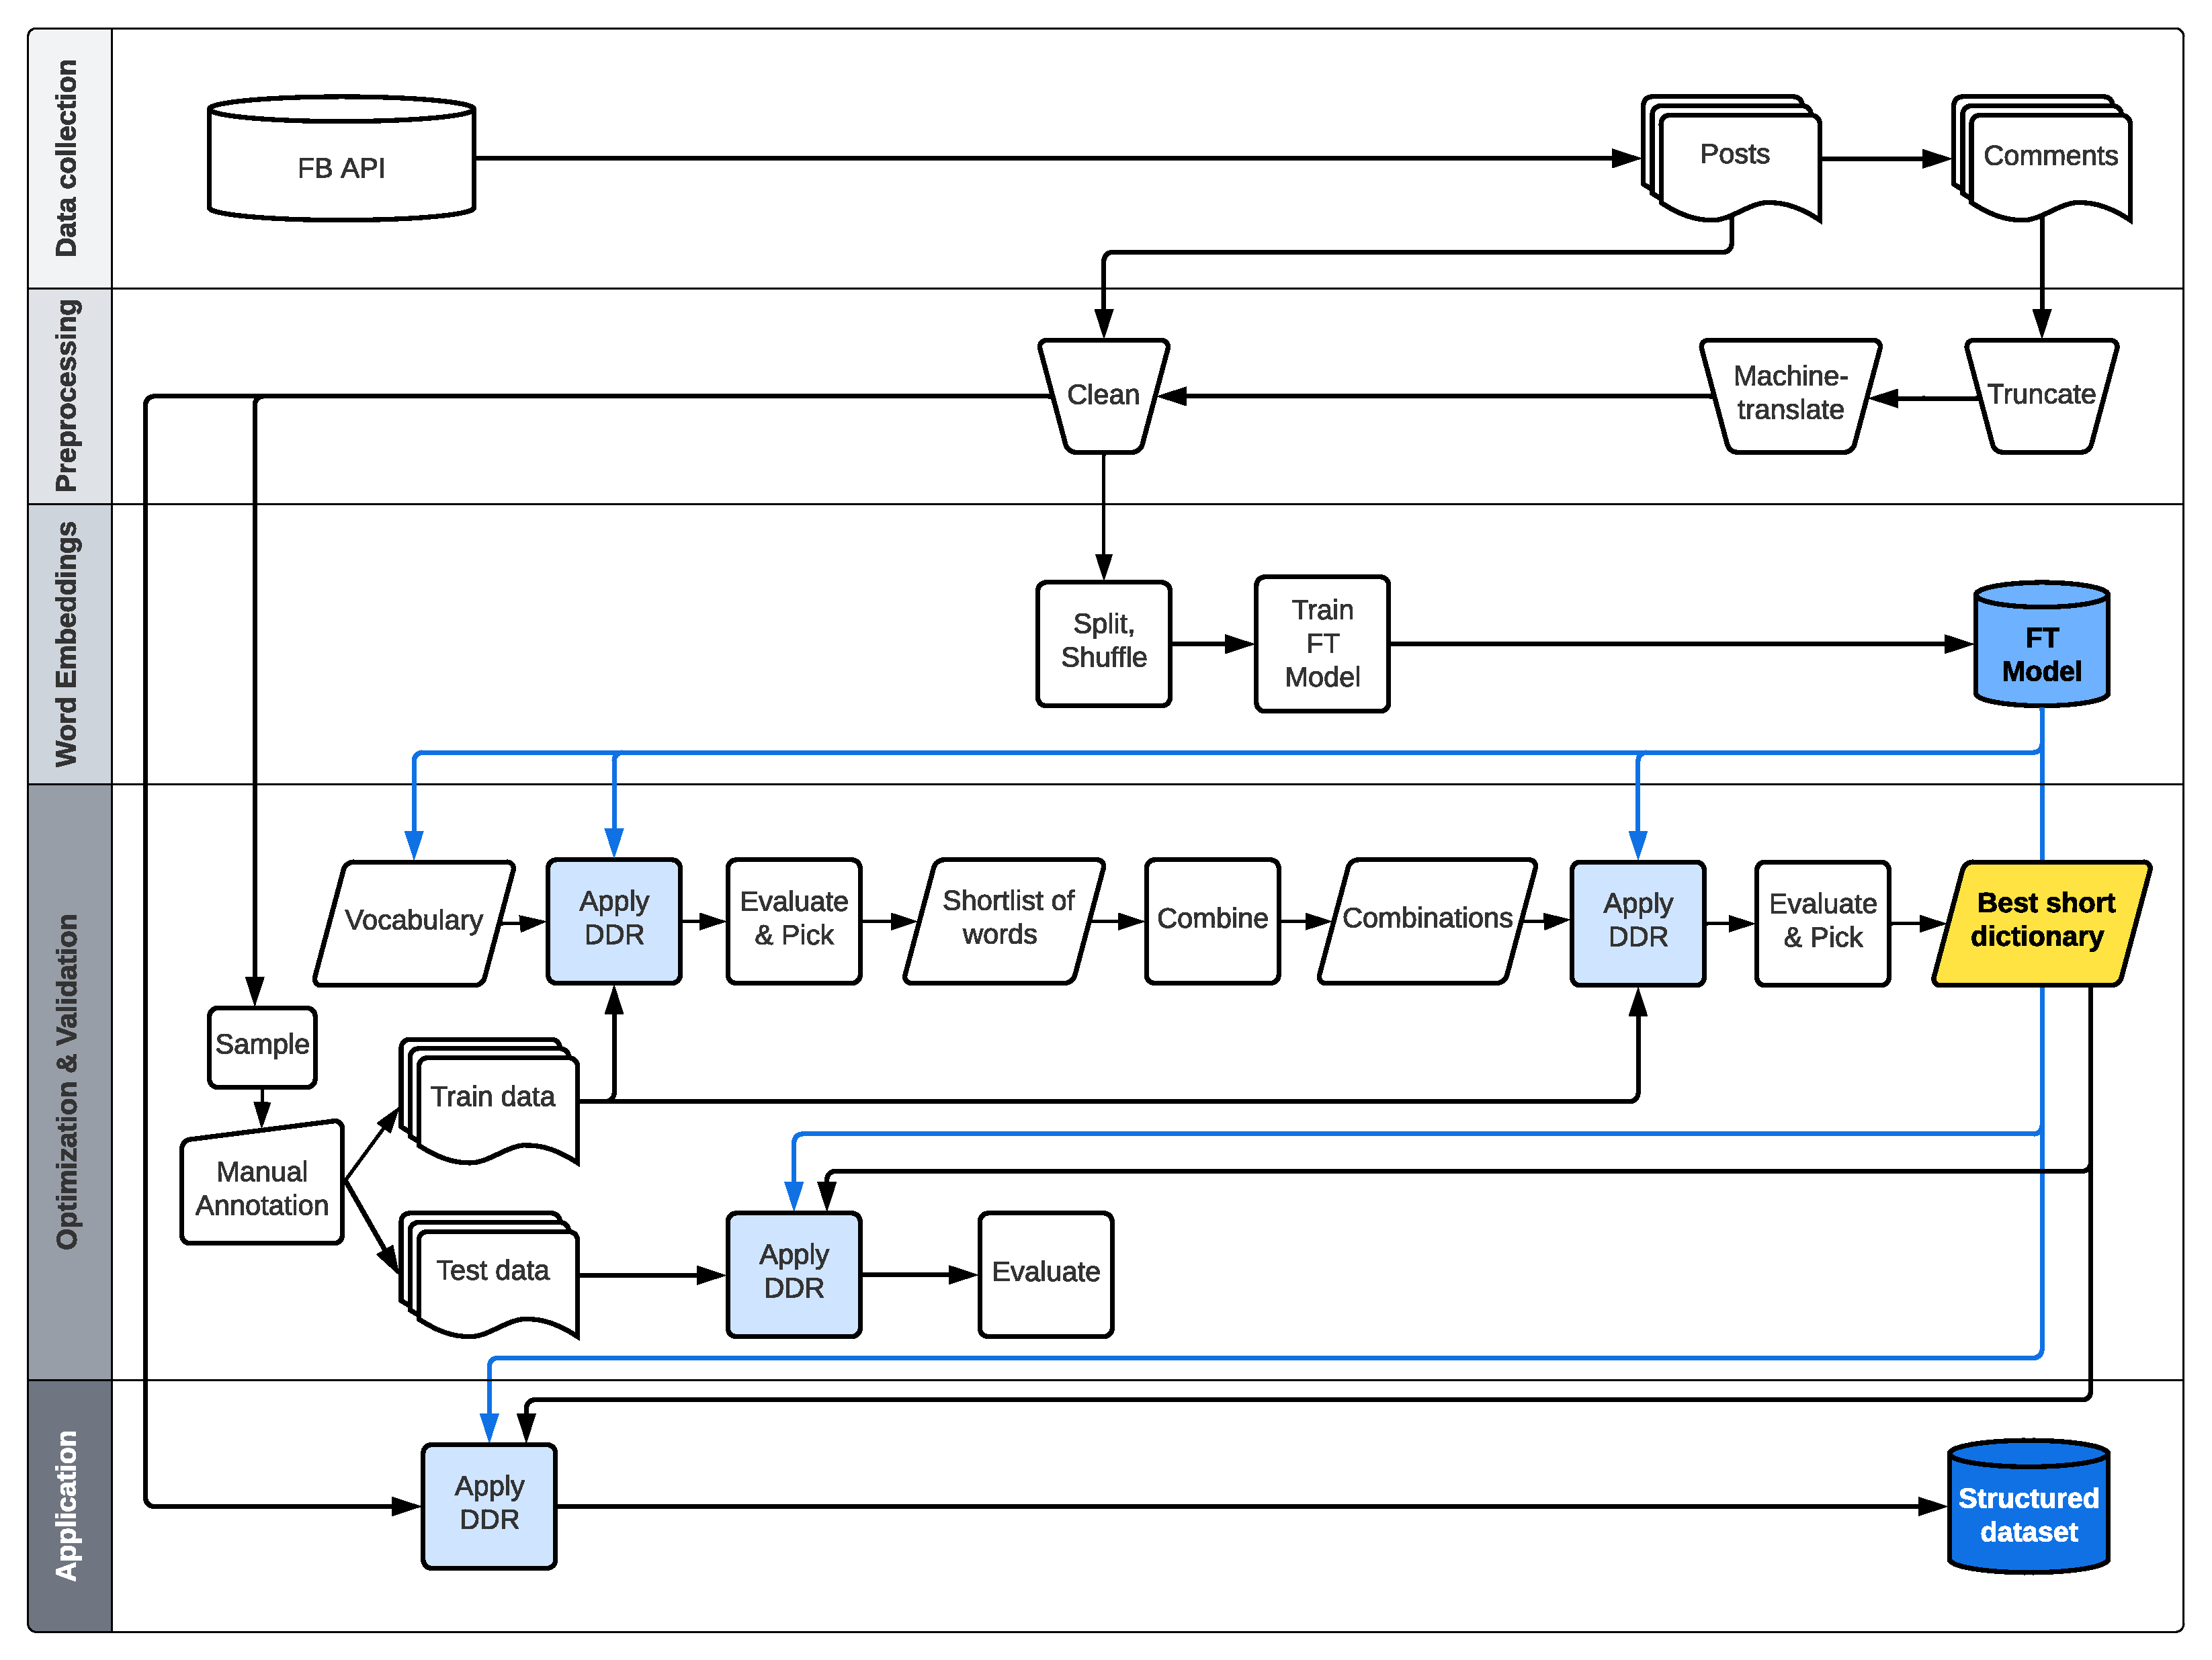
\includegraphics{plots/pipeline_CCR_paper_20230516.pdf}

}

\caption{Pipeline for Optimizing and Applying the DDR Measurement}

\end{figure}

\hypertarget{fasttext-model}{%
\subsubsection{\texorpdfstring{\emph{FastText}
Model}{FastText Model}}\label{fasttext-model}}

I trained a custom \emph{fastText} word embedding model (Bojanowski et
al. 2017) using the comprehensive corpus of German comments and
German-language posts, including translations. Word embeddings represent
the semantic relations between words in a multidimensional vector space
(Mikolov et al. 2013). These vector representations are produced by
machine learning algorithms trained on extensive text corpora. These
rely on the assumption that words of similar meaning repeatedly occur in
similar contexts (Mikolov et al. 2013). \emph{FastText} models,
distinguished from other embeddings, excel in handling social media
texts as they are robust against misspellings, can generate vectors for
out-of-vocabulary words, and perform well on morphologically rich
languages. These capabilities are achieved by segmenting words into
n-grams of characters, and inferring embeddings for these sub-word
snippets as well (Bojanowski et al. 2017).

For the task in this research, I preferred a custom-trained word
embedding model. Pre-trained, off-the-shelf models are typically sourced
from curated texts like Wikipedia, which lack authentic expressions of
populism. In addition, pre-trained models miss the meaning of terms with
current relevance. This seems particularly relevant in the context of
the COVID-19 crisis, which resulted in a whole vocabulary of new words.

The documents used for training underwent cleaning processes detailed in
Appendix B, were segmented into sentences using the \emph{quanteda}
(Benoit et al. 2018) tokenizer, and then randomized. After filtering
duplicates and sentences containing fewer than 5 words, the model
training dataset encompassed 3,564,352 lines of text.

The model was trained on a local machine (Intel(R) i7-8565U CPU @
1.80GHz, 4 cores, 8 threads, 16 GB RAM, no GPU) utilizing the
\emph{fastrtext} R-package (Benesty 2019). I chose the skipgram method
to train a model 200 dimensions, with the following hyperparameters: 20
epochs, learning rate .1, bucket size 2,000,000, context window size 7,
maximum n-gram length 6, minimum n-gram length 3, and set a minimum word
count threshold of 10 for inclusion in the vocabulary. The training
completed within less than 2 hours, yielding a vocabulary of 89,309
terms.

To evaluate the model's quality via face validity, I reviewed results
from several nearest neighbor queries using political terms. For the
formal validation, I focused on output validity, as reported in the main
article. The model, along with the replication materials, is included in
the replication repository: \url{https://osf.io/d4qng/}.

\hypertarget{optimizing-the-ddr-measurement}{%
\subsubsection{Optimizing the DDR
Measurement}\label{optimizing-the-ddr-measurement}}

The main article details the DDR method, validation data, and evaluation
strategy. This section focuses on outlining the steps taken to identify
an optimal DDR dictionary specifically geared toward capturing
user-generated expressions of populism. The objectives were threefold:
First, the dictionary should be \emph{inductively} derived, reflecting
genuine user-generated expressions of populism. At the same time,
second, the dictionary should be \emph{theory-driven}, reflecting core
dimensions of populism. Third, the resulting measurement should be
\emph{comparable}, maximizing F1 scores across all countries. The R-code
to replicate these steps is presented in the vignette `from text to
measurement' within my R-package \emph{dictvectoR} (Thiele 2022b). Due
to copyright restrictions, the original Facebook text data cannot be
shared. The data provided in the replication repository includes the
scores from applying the DDR measurement and shareable data.

Commencing with the 89,309 terms in the \emph{fastText} model's
vocabulary, I excluded the least common 10\% of words and stop-words.
Each word's cosine similarity to the average representation of two
corpora was computed: Firstly, to the average representation of all
comments tagged as populist in the training corpus and secondly, to the
representation of all non-populist comments in the training dataset.
Additionally, I computed the score difference, facilitated by
\texttt{dictvectoR::find\_distinctive()}. This initial process provided
rough indicators for words potentially enhancing the recall and
precision of the DDR score. I used the product of the populism
similarity and distinctiveness scores to narrow down the list of words
to 3,000 words. Multiword expressions frequently used in a random 50\%
subset of the corpus were added using
\texttt{dictvectoR::add\_multiwords()}. Multiword expressions are
important in populist communication, as they are used to construct in-
and out-groups (e.g., `wir steuerzahler') and distinguish neutral from
populist meanings of words. Next, F1 scores for each individual term
were obtained, by treating each term as one-term-dictionary in the DDR
and the annotated train sample for evaluation.
\texttt{dictvectoR::get\_many\_F1s()} takes care of this task. Highly
similar terms were dropped, keeping the best performing with
\texttt{dictvectoR::remove\_similar\_words()}.

Next, the words were reviewed manually. First, words were coarsely coded
for relevance. Highly idiosyncratic word combinations and
near-duplicates were dropped. Second, the remaining list of 287 terms
was annotated using a more nuanced classification. Terms were annotated
as referring to `elites', `the people', or some kind or `relation'
between those two antagonists. For `elites' I further annotated
subcategories. The terms annotated as `relation', contained the
subcategories `blaming', `manipulation', `sovereignty', `damaging', and
`unaccountable'. These categories were built inductively from the
identified words but reflect theoretical key dimension of populist
discourse. From each of the three dimensions, the 15 best performing
terms were selected.

Using combinatorics and random sampling, 2.9 million different
combinations of these 45 words were obtained. Dictionary lengths between
three to fifteen words were allowed, with at least one word per
dimension. The number of combinations was limited by randomly picking up
to 100 combinations for each number of words per dimension combination.
For example, instead of featuring all 3,003 combinations of length 5
from the 15 terms for `elites', only 100 were sampled and combined with
all combinations for the other dimensions.
\texttt{dictvectoR::get\_combis()} provides this function. The
performance of the DDR measurements for each of the 2.9 million
combinations was assessed by their F1 in predicting the human annotation
in the train data. For the 10k best-performing combinations, F1 scores
were computed additionally for each country. To evaluate consistency
across countries, the 8th root of the product of the overall F1 score
times all seven country F1 scores was calculated. The dictionary that
maximized F1 most consistently on the train data was selected. A manual
inspection, using the annotated subcategories, deemed that dictionary
conceptually balanced and convincing. This dictionary and the validation
results are documented in the main text.

\hypertarget{additional-equivalence-assessment}{%
\subsubsection{Additional Equivalence
Assessment}\label{additional-equivalence-assessment}}

In addition to the validation documented in the main text, I inspected
the importance of each single dictionary term for the measurement
performance across countries. To quantify the impact of each single
term, a list of 12 dictionaries was created where each dictionary left
out one of the 12 terms in the selected DDR dictionary. Each of these
`incomplete' dictionaries was used to predict populism in the (1)
combined test \& train validation sample, and (2) the test sample alone,
and a F1 score calculated, as described in the main article. To assess
deteriorated or improved performance, I inspect the difference between
the F1 scores for the `incomplete' and the complete DDR-dictionary. The
heat-map in Figure C2 documents how leaving out one of the 12
DDR-dictionary terms (y-axis) improves (positive values; light-yellow)
or deteriorates (negative values; dark-blue) the F1 score, compared to
the complete dictionary performance in predicting populism in the test
and train data (left grid) and test sample alone (right grid).

The performance of an ideal measurement would (a) not decrease strongly
by leaving out one term, (b) would exhibit a balanced pattern of term
importance, and (c) would exhibit similar patterns across all countries.
The heat-map in Figure C2 shows that the selected DDR-dictionary comes
close to achieving these goals for the untranslated Austrian and German
corpora: The differences there are relatively small
(\textless\textbar.03\textbar) and do not show outlying terms for both
the combined data, as well as the test data alone. Similarly homogeneous
patterns emerge for the Netherlands, and UK. The pattern is less
balanced for France, Sweden, and Italy. For example, leaving out the
term ``sogenannte experten'' decreases the performance on the French
train \& test corpus by -.05, and in likewise by -.05 in the Italian
test corpus. These patterns illustrate that country-contexts continue to
have an impact on the meaning of words, even after machine translation
(Licht and Lind 2023, 20), and hence affect measurement performance and
equivalence. The patterns are more imbalanced in the test data, which
seems concerning. However, it must be noted that these imbalances are
partly driven by the low number of true positives in the Italian (n= 22,
26\%) and Swedish (n=27; 32\%) test data, which is below the mean share
of true positives in population test dataset (40\%). As discussed in the
main article, the careful inspection of the DDR measurement raises
questions about its comparability across countries. Appendix E presents
a robustness check of the comparative findings resulting from the
regression analysis.

\begin{figure}

{\centering 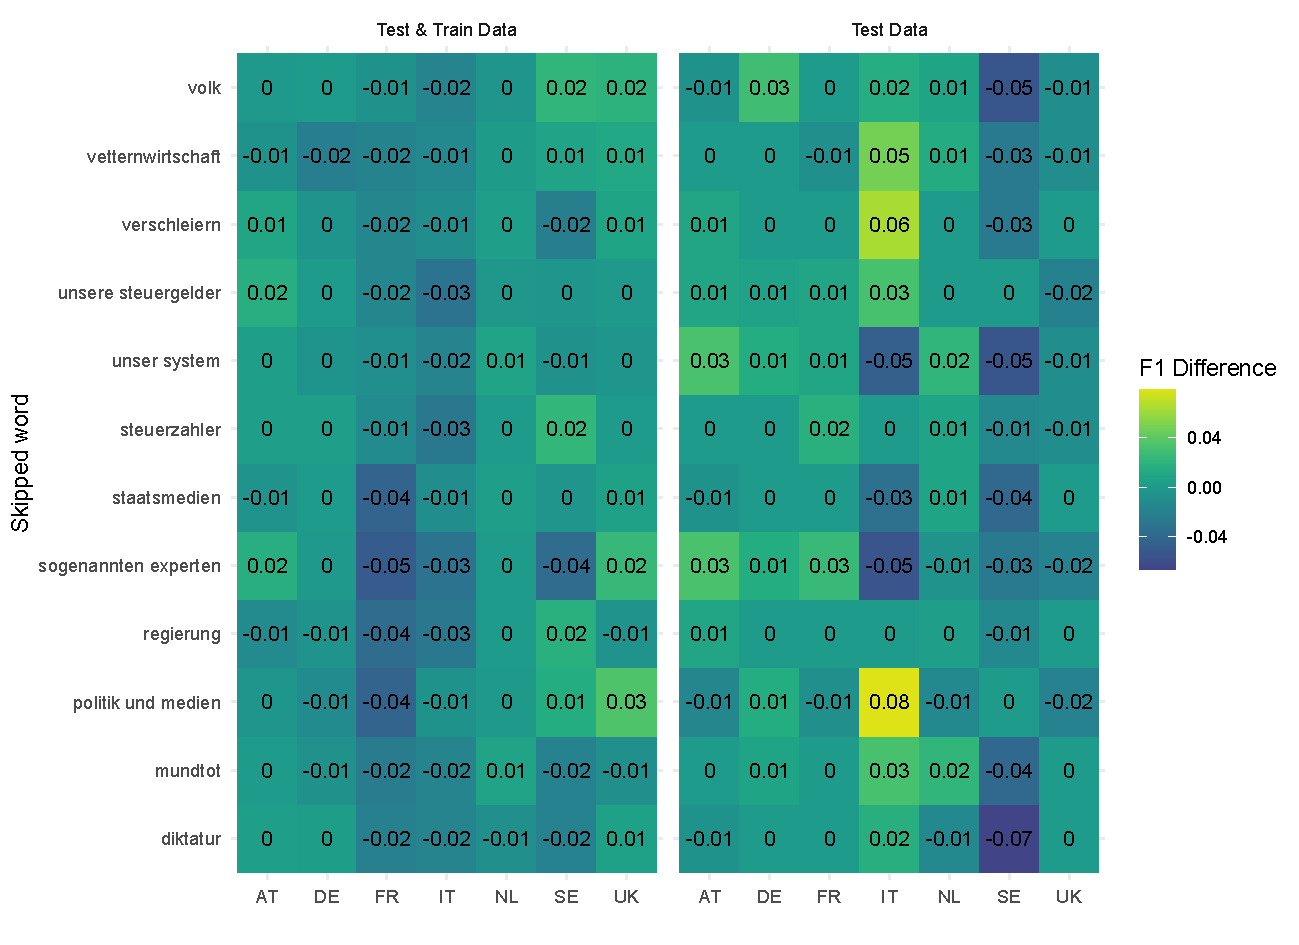
\includegraphics{plots/heatmap_skip_words_20231129.pdf}

}

\caption{Changes in F1 when leaving out single DDR-dictionary terms by
country}

\end{figure}

\newpage
\renewcommand{\thefigure}{D\arabic{figure}}
\renewcommand{\thetable}{D\arabic{table}}
\setcounter{figure}{0}
\setcounter{table}{0}

\hypertarget{appendix-d}{%
\subsection{Appendix D}\label{appendix-d}}

\hypertarget{dictionaries}{%
\subsubsection{Dictionaries}\label{dictionaries}}

The subsequent tables document the multilingual dictionaries used for
capturing references to \emph{COVID-19,} COVID-19 containment policies
(\emph{Measures),} lifting of restrictive policies (\emph{Easing)}, as
well as \emph{Experts} and the \emph{Government}. Notably, the
dictionaries for the first three categories share overlap, functioning
as sub-categories of one another: All terms within \emph{Measures} are
encompassed within \emph{COVID-19}, and all terms within \emph{Easing}
are included in \emph{Measures}.

The development of these dictionaries commenced with a manual
translation derived from an existing German dictionary (Thiele 2022a),
complemented by the utilization of translation websites (linguee.de;
context.reverso.net) providing contextualized translations. Each term's
suitability was determined through careful consideration of suggested
translations and contextual relevance. Ambiguous terms were excluded.
Subsequently, country-specific \emph{fastText} models were trained,
following the methodology detailed in Appendix C, utilizing the
non-translated post corpora. These models were employed to retrieve the
20 nearest neighbors for each term. The obtained results underwent a
secondary manual inspection, cross-referenced with context-sensitive
translation websites (linguee.de; context.reverso.net). Furthermore, I
used \texttt{quanteda::keywords-in-context()} to inspect the contextual
use of the identified keywords within the analyzed corpus. Both sources
of information were instrumental in supplementing the list of keywords,
increasing the precision of the dictionary, and inferring wildcard
placements.

The \emph{Government} dictionaries maintain case sensitivity and were
applied to the non-lowercased corpora. To enrich these dictionaries, I
compiled the names of the members of each country's national cabinets at
the time of analysis, occasionally excluding too common family names.
The German and Austrian dictionaries are identical except for their
\emph{Government} dictionary. All dictionaries are provided in a
machine-readable format in the replication repository.

{
\begin{spacing}{.9}
\fontsize{8}{9}\selectfont 
\begin{longtable}[]{@{}
  >{\raggedright\arraybackslash}p{.09\linewidth}
  >{\raggedright\arraybackslash}p{.12\linewidth}
  >{\raggedright\arraybackslash}p{.71\linewidth}@{}}
\caption{Dictionaries.} \\
\toprule\noalign{}
\textbf{Language} & \textbf{Concept} \newline \emph{(n words)} & \textbf{Words}\textsuperscript{a} \\
\midrule\noalign{}
\endhead
%\bottomrule\noalign{}
\endlastfoot 
\begin{minipage}[t]{\linewidth}\raggedright
DE\\
\strut \\
\strut
\end{minipage} & COVID-19 (124) & *ansteck*, *ausgangssperre*,
*cluster*, *geimpft*, *immunisier*, *impf*, *infektion*, *infizier*,
*lockdown*, *lockerung*, *maske*, *maskenpflicht, *maßnahme*, *pandemi*,
*quarantäne*, *reisebeschränkung*, *reiseverbot*, *schnelltest*,
*testpflicht*, *vakzin*, *viren*, *virus*, abstandsregel*, angesteckt*,
antigen*, antikörper*, arzneimittelbehörde, astra*,
ausgangsbeschränkung*, ausreisetestpflicht, biontech*, blutgerinnsel,
blutgerinnseln, bundesgesundheitsminister, corona*, cov, covid*, delta,
dosen, durchimpfung*, einreise*, einreisebeschränkung*,
einreisebestimmungen, einreisestop*, einreiseverbot*, epidemie*,
erkranken, erkrankung*, erreger, fallzahl*, ffp*, freitest*, gelockert,
genesungen, gesundheitsexperte, gesundheitsminister, gesundheitssystem*,
getestet*, ghebreyesus, gurgelt, herdenimmunität, home*office,
homeoffice*, hospitalisierungen, hygiene, hygieneregeln, impfpflicht,
intensivmedizinisch, intensivpatienten, intensivstationen, inzidenz*,
kontaktbeschränkungen, kontaktpersonen, kontaktverbot*, kontrollen,
körpernahe, lombardei, lungenkrankheit, masken*pflicht, massentest*,
mindestabstand, moderna, mutante, mutanten, mutation, mutationen,
neuinfektion*, notfallzulassung, öffnet, öffnungsschritt*, patienten,
pcr*, pfizer*, pharmaunternehmen, präsenzunterricht*, regeln,
reisewarnung*, reproduktionszahl*, risikogebiet*, risikogruppen, rki,
sars*, sauerstoff, schulöffnung*, schulschließung*, schutzmaske*,
schutzregel*, selbsttest*, social distanc*, sperrzone, spitalspatienten,
stark eingeschränkt, superspread*, tests, teststraße*, teststrategie*,
ungeimpft*, weiter eingeschränkt, weltgesundheitsorganisation, who,
wieler, wuhan, zeneca, zweite* welle \\ \cline{2-3}

& Measures (69)\textsuperscript{b} & *ausgangssperre*, *geimpft*,
*impf*, *lockdown*, *lockerung*, *maske*, *maskenpflicht, *maßnahme*,
*quarantäne*, *reisebeschränkung*, *reiseverbot*, *schnelltest*,
*testpflicht*, *vakzin*, abstandsregel*, antigen*, arzneimittelbehörde,
astra*, ausgangsbeschränkung*, ausreisetestpflicht, biontech*, dosen,
durchimpfung*, einreise*, einreisebeschränkung*, einreisebestimmungen,
einreisestop*, einreiseverbot*, ffp*, freitest*, gelockert, getestet*,
gurgelt, home*office, homeoffice*, hygiene, hygieneregeln, impfpflicht,
kontaktbeschränkungen, kontaktpersonen, kontaktverbot*, kontrollen,
masken*pflicht, massentest*, mindestabstand, moderna, notfallzulassung,
öffnet, öffnungsschritt*, pcr*, pfizer*, pharmaunternehmen, regeln,
reisewarnung*, risikogebiet*, schulöffnung*, schulschließung*,
schutzmaske*, schutzregel*, selbsttest*, social distanc*, sperrzone,
stark eingeschränkt, tests, teststraße*, teststrategie*, ungeimpft*,
weiter eingeschränkt, zeneca \\ \cline{2-3}

& Easing (5)\textsuperscript{c} & *lockerung*, gelockert, öffnet,
öffnungsschritt*, schulöffnung* \\ \cline{2-3}

& Experts (50) & *arzt, *ärzt*, *expert*, *forschen*, *forschende*,
*forscher*, *forschung*, *ologe, *ologen, *ologin, *professor*,
*spezialist*, *studie, *studien, *studiendaten*, *studienergebnis*,
*universität*, *wissenschaft*, anästhes*, apotheker, charité, drosten,
endokrinolog*, epidemiolog*, ethikrat*, fachleute*, fda, ghebreyesus,
immunolog*, impfkommission, infektiolog*, institut*, intensivmedizin,
intensivmediziner, johns hopkins, mediziner, meduni, mikrobiolog*,
pneumolog*, psycholog*, rki, robert koch, stiko, uni,
universitätsklinik*, vakzinolog*, virolog*, weltgesundheitsorganisation,
who, wieler \\ \cline{2-3}

& Government - AT (39)\textsuperscript{d} &
*inisterin Aschbacher, *kanzler*,
*koalition*, *minister*, *minister?, *ministerium*, *regierung*,
Anschober, Blümel, Brüssel, Christine Aschbacher, Edtstadler, EU
Kommission*, eu* Kommission*, Europäische* Kommission*, Faßmann,
Gewessler, Kabinett*, Kanzler*, Kocher, Kogler, Kommissionchefin,
Kommissionspräsidentin, Köstinger, Kurz, Lunacek, Magnus Brunner,
Minister, Ministerin, Ministerium*, Ministerrat*, Mückstein, Nehammer,
Raab, Regierung*, Schallenberg, Schramböck, Tanner, Zadic \\ \cline{2-3}

& Government - DE (38)\textsuperscript{d} &
*inisterin Schulze, *kanzler*, *koalition*,
*minister*, *minister?, *ministerium*, *regierung*, ?on der Leyen,
Altmaier, Barley, Brüssel, EU Kommission*, eu* Kommission*, Europäische*
Kommission*, Giffey, Heil, Helge Braun, Kabinett*, Kanzler*, Kanzleramt*
Braun, Karliczek, Klöckner, Kommissionchefin, Kommissionspräsidentin,
Kramp Karrenbauer, Lambrecht, Maas, Merkel*, Minister, Ministerin,
Ministerium*, Ministerrat*, Regierung*, Scheuer, Scholz, Seehofer,
Spahn, Svenja Schulze \\ \cline{1-3}

EN & COVID-19 (77) & *cluster*, *easing*, *hotspot*, *immuni*,
*infect*, *lockdown*, *pandemi*, *quarantine*, *vaccin*, *vaccinated*,
*vaxx*, *virus*, antibod*, astra*, ban family visit*, ban visit*,
biontech*, cases, combat coronavirus, contact tracing, containment
measure*, corona*, coronavirus measure*, coronavirus safety measure*,
coronavirus test*, covid measure*, covid test*, covid*, curfew,
distancing, dose*, doses, eases, easing, epidemic, epidemic measure*,
fatalit*, fight against covid, fight coronavirus, government response*,
health verification*, health* measure*, healthcare, isolat*, jab,
lifting, limit* travel*, major incident, mask*, mass test*, measure*
taken, measure* to combat, measure* to fight, moderna, outbreak, pcr*,
pfizer*, re?open*, reopening, restrictions, sanitiser, sars*, stem
spread, stem the spread, strict* measure*, superspread*, test and trace,
test positive, tested on covid, tested positive, testing, tougher
measure*, tracing app, transmission, travel ban*, travel restrictions,
wuhan \\ \cline{2-3}
& Measures (60)\textsuperscript{b} & *easing*, *immuni*, *lockdown*,
*quarantine*, *vaccin*, *vaccinated*, *vaxx*, astra*, ban family visit*,
ban visit*, biontech*, combat coronavirus, contact tracing, containment
measure*, coronavirus measure*, coronavirus safety measure*, coronavirus
test*, covid measure*, covid test*, curfew, distancing, dose*, doses,
eases, easing, epidemic measure*, fight against covid, fight
coronavirus, government response*, health verification*, health*
measure*, isolat*, jab, lifting, limit* travel*, major incident, mask*,
mass test*, measure* taken, measure* to combat, measure* to fight,
moderna, pcr*, pfizer*, re?open*, reopening, restrictions, sanitiser,
stem spread, stem the spread, strict* measure*, test and trace, test
positive, tested on covid, tested positive, testing, tougher measure*,
tracing app, travel ban*, travel restrictions \\ \cline{2-3}
& Easing (6)\textsuperscript{c} & *easing*, eases, easing, lifting,
re?open*, reopening \\ \cline{2-3}
& Experts (28) & doctor*, endocrinolog*, epidemiolog*, ethic* adviser,
expert*, extrapolate, fda, finds, ghebreyesus, health professional,
immunolog*, institute, johns hopkins, microbiolog*, pharmacists,
physician*, professor, psycholog*, public health england, pulmonolog*,
research*, scien*, specialist*, study, survey, technique, virolog*,
world health organi?ation \\ \cline{2-3}
& Government (48)\textsuperscript{d} & Alister Jack, Barclay, Ben
Wallace, Brandon Lewis, Braverman, Brussels, Buckland, Coffey,
commission president, Commission President, Dowden, EU commission*,
European commission, Eustice, Gove, government, Government, Hancock,
Hart, Jenrick, Johnson, Kwarteng, Liz Truss, Lord Frost, Mark Spencer,
Michael Ellis, Milling, minister, Minister, ministry, Ministry, of Bowes
Park, Patel, PM, prime minister Boris, Prime Minister Boris, Prime
Minister Johnson, Raab, Rees Mogg, secretary, Secretary, Shapps, Sharma,
Sunak, Trevelyan, UK prime minister, UK Prime Minister, Williamson \\ \cline{1-3}

FR & covid-19 (63) & *anticorps, *autotest*, *épidémie, *incidence,
*virus, antigéniques, astra*, biontech*, cas, cluster, confin,
confinement, confinements, contag*, contamin*, contre la *pandemie,
contre le *virus, contre le covid, corona*, couvre feu, cov, covid*,
décision* difficil*, déconfinement, doses, écol* ferm*, événements
annulés, fermés, fermeture*, ffp*, gestes barrières, hospitalisés,
immunis*, immunitaire, immunité, infect*, inocul*, masque*, mesures
barrières, mesures de confinement, mesures le covid, mesures
restrictives, moderna, nouvell* mesur*, pand*mie, pcr, pfizer*,
pharmaceutique, quarantaine, reconfinement, relâchement, réouverture,
restrictions, rouvert, sars*, stopcovid, télétravail*, test*,
transmission, vaccin*, variant, variants, wuhan \\ \cline{2-3}

& Measures (41) & *autotest*, antigéniques, astra*, biontech*, confin,
confinement, confinements, contre la *pandemie, contre le *virus, contre
le covid, couvre feu, décision* difficil*, déconfinement, doses, écol*
ferm*, événements annulés, fermés, fermeture*, ffp*, gestes barrières,
inocul*, masque*, mesures barrières, mesures de confinement, mesures le
covid, mesures restrictives, moderna, nouvell* mesur*, pcr, pfizer*,
pharmaceutique, quarantaine, reconfinement, relâchement, réouverture,
restrictions, rouvert, stopcovid, télétravail*, test*, vaccin* \\ \cline{2-3}

& Easing (4)\textsuperscript{c} & déconfinement, relâchement,
réouverture, rouvert \\ \cline{2-3}

& Experts (30) & *ologiste, *ologue, *ologues, chercheur*, conseil de la
santé, endocrinolog*, épidémiolog*, essai* clinique*, étude*, expert*,
fda, ghebreyesus, hcsp, immunolog*, infectiolo*, institut, johns
hopkins, médecin, médecins, microbiolog*, oms, organisation mondiale de
la santé, pneumolog*, professionnel* de santé, psycholog*, scien*,
spécialist*, traitement, université, virolog* \\ \cline{2-3}

& Government (40)\textsuperscript{d} & Bachelot, Belloubet, Blanquer,
Borne, Bruxelles, Buzyn, Castex, Collomb, Commission européenne,
Darmanin, Denormandie, Dupond-Moretti, Dupond Moretti, Edouard Philippe,
Flessel Colovic, Girardin, Gourault, gouvernement, Hulot, Le Drian, Le
Maire, Lecornu, Macron, Matignon, Mézard, ministère, ministre*,
Montchalin, Nyssen, Parly, Pénicaud, Pompili, président de la
République, président Emmanuel, président français, président Macron,
présidente de la Commission européenne, Travert, Véran, Vidal \\ \cline{1-3}

IT & COVID-19 (70) & *antigen*, *contag*, *epidemi*, *immun*,
*incidenz*, *infett*, *infez*, *pandemi*, *vaccin*, *vaccina*, *virale,
*virus*, allentament*, anti coronavirus, anti covid, anti virus,
anticorp*, astra zeneca, astrazeneca, biontech*, casi, contenere i*,
contenere la, contenimento, coprifuoco, coronavir*, cov, covid*,
decessi, delta, distanziamento, dosi, ffp*, guariti, impone, isolament*,
lockdown, lotta alla pandemia, mascherin*, misura, misure, misure
restrittive, misure rigide, morti, nuova stretta, passaporto sanitario,
pfizer, provvedimenti, quarantena, restrizioni, riaperture, riapre,
ricoverati, sars*, scuole chiuse, sintomi, superspreader, telelavor*,
test, trasmissibilità, trombosi, una stretta, variante, virologi,
virologia, wuhan, zona arancione, zona gialla, zona rossa, zone rosse \\ \cline{2-3}

& Measures (43)\textsuperscript{b} & *antigen*, *vaccin*, *vaccina*,
allentament*, anti coronavirus, anti covid, anti virus, astra zeneca,
astrazeneca, biontech*, contenere i*, contenere la, contenimento,
coprifuoco, distanziamento, dosi, ffp*, impone, isolament*, lockdown,
lotta alla pandemia, mascherin*, misura, misure, misure restrittive,
misure rigide, nuova stretta, passaporto sanitario, pfizer,
provvedimenti, quarantena, restrizioni, riaperture, riapre, scuole
chiuse, telelavor*, test, trombosi, una stretta, zona arancione, zona
gialla, zona rossa, zone rosse \\ \cline{2-3}
 
& Easing (3)\textsuperscript{c} & allentament*, riaperture, riapre \\ \cline{2-3}

& Experts (39) & agenzia italiana del farmaco, aifa, anestes*, autorità
sanitarie, borrelli, commissione sanitaria, dott, dottore*,
endocrinolog*, epidemiolog*, espert*, farmacisti, fda, fondazione,
ghebreyesus, immunolog*, infettivolog*, institut*, johns hopkins,
magrini, medici, medico, microbiolog*, oms, organizzazione mondiale
della sanità, pneumolog*, professore*, psicolog*, ricerc*, ricerca,
ricercatore, ricercatori, ricercatrice, scien*, specialist*, studi,
studio, università, virolog* \\ \cline{2-3}

& Government (59)\textsuperscript{d} & *inistro Bianchi, ?onsiglio dei
?inistri, ?residente del ?onsiglio, Amendola, Azzolina, Bellanova,
Boccia, Bonafede, Bonetti, Brunetta, Bruxelles, Carfagna, Cartabia,
Catalfo, Cingolani, Colao, commissione europea, Commissione europea,
Commissione Europea, Consiglio dei ministri, Conte, D'Incà, D Incà,
Dadone, Daniele Franco, De Micheli, Di Maio, Draghi, Fioramonti,
Fraccaro, Franceschini, Garavaglia, Garofoli, Gelmini, Giorgetti,
Giovannini, governo, Governo, Gualtieri, Guerini, Lamorgese, Manfredi,
Messa, minister?, Minister?, ministr?, Ministr?, Orlando, Patrizio
Bianchi, Patuanelli, Pisano, premier, presidente della ?ommissione
?uropea, presidente della ?ommissione Ue, Provenzano, Sergio Costa,
Spadafora, Speranza, Stefani \\ \cline{1-3}

NL & COVID-19 (110) & *antigeen*, *antilicham*, *besmet*, *inent*,
*infect*, *lockdown*, *masker*, *metermaatregel*, *pandemie*,
*quarantain*, *reisverbod*, *vaccin*, *virus*, afstand*,
anderhalvemetermaatschap*, anderhalvemeterregel,
anderhalvemetersamenlev*, astra*, avondklok*, avondklokken,
avondklokrellen, basisschool dicht, beperkende maatregel*, bezoekregel*,
bijwerkingen, biontech*, cluster*, code rood, corona, corona maatregel*,
corona*, coronabeleid, coronagevallen, coronamaatregelen, coronaregels,
coronatesten, coronatests, coronawet, covid*, doses, ema, epidemie*,
farmaceut, farmaceuten, ffp*, gaan dicht, gemuteerde,
geneesmiddelenbureau, geprikt, gevaccin*, gezondheidsraad,
gezondheidszorg*, groepsimmuniteit*, heropenen, injectie, inreisregel*,
kunnen open, maatregel*, maatregel* om de verspreiding, maatregel* tegen
het coronavirus, masker*, moderna, mondkapje*, mutatie, nieuwe
maatregel*, openingsplan, patiënten, pcr*, pfizer*, prikken, reisadvie*,
reisbeperk*, reisverbod*, reproductiegetal*, restaurants dicht,
risicogebied*, rivm, sars*, scholen dicht, sneltest*, sterfgevallen,
steunmaatregelen, strenge* maatregel*, terrassen open*, testen*,
teststrategie, teststraten, thuisblijven, thuiswerken, variant,
varianten, veiligheidsmaatregel*, verpleegafdelingen, verplicht,
versoepeld, versoepelen, versoepeling, versoepelingen,
virusmaatregelen*, voorlopig dicht, weer open*,
wereldgezondheidsorganisatie*, who, winkels dicht, wuhan, zelftest*,
ziekenhuis, ziekenhuisopnames, ziekenhuispersoneel, zorgsysteem* \\ \cline{2-3}

& Measures (58)\textsuperscript{b} & *antigeen*, *inent*, *lockdown*,
*masker*, *quarantain*, *reisverbod*, *vaccin*, afstand*,
anderhalvemeterregel, astra*, avondklok*, avondklokken, avondklokrellen,
bezoekregel*, biontech*, coronabeleid, coronamaatregelen, coronaregels,
coronatesten, coronatests, coronawet, doses, ema, farmaceut, ffp*,
geprikt, gevaccin*, heropenen, injectie, inreisregel*, kunnen open,
maatregel*, masker*, moderna, mondkapje*, openingsplan, pcr*, pfizer*,
prikken, reisadvie*, reisbeperk*, reisverbod*, risicogebied*, sneltest*,
steunmaatregelen, terrassen open*, testen*, teststrategie, teststraten,
thuiswerken, verplicht, versoepeld, versoepelen, versoepeling,
versoepelingen, virusmaatregelen*, weer open*, zelftest* \\ \cline{2-3}
 
& Easing (10)\textsuperscript{c} & heropenen, kunnen open,
openingsplan, steunmaatregelen, terrassen open*, versoepeld,
versoepelen, versoepeling, versoepelingen, weer open* \\ \cline{2-3}

& Experts (37) & *deskundige*, *expert*, *loog, *ologen, *onderzoek,
*onderzoek*, *onderzoeken, *onderzoeker*, *specialist*, *studie,
*studies, *wetenschap*, arts*, dokt?r*, epidemiolog*, fda, ggd,
ghebreyesus, hogeschool, hooglera*, immunolog*, istitut*, johns hopkins,
longarts*, microbiolog*, nvwa, planbureau*, professor*, psycholog*,
rijksinstituut, rivm, scp, studieresultaten, universiteit, virolog*,
wereldgezondheidsorganisatie, who \\ \cline{2-3}

& Government (46)\textsuperscript{d} & *inister Bruins, *inister
Schouten, *minister, *minister?, ?an Ark, ?an Engelshoven, ?an
Nieuwenhuizen, ?an Rijn, ?an Veldhoven, ?e Jonge, Barbara Visser,
Bijleveld, Blok, Bruno Bruins, Brussel, Carola Schouten,
Commissievoorzitter, de Bruijn, Europese Commissie, Grapperhaus, Henk
Kamp, Hoekstra, Kaag, kabinet*, Kabinet*, Knapen, Koolmees, Minister,
ministerie, Ministerie, ministerraad, Ollongren, overheid, Overheid,
premier, Premier, Raymond Knops, regering*, Regering*, Rutte, Sander
Dekker, Slob, van Nieuwenhuizen, van t Wout, Wiebes, Zijlstra \\ \cline{1-3}

SE & COVID-19 (110) & *epidemi*, *infekt*, *karantän*, *lockdown*,
*masker*, *pfizer*, *reseförbud*, *reserestriktion*, *vaccin*, *virus*,
antigen*, antikropp*, astra*, besöksförbud, biontech*, biverkningar,
blodproppar, bromsa* spridning*, corona strategi, corona*, coronaåret,
coronapandemin, coronarestriktioner*, coronasmittad, coronasmittade,
coronastrategi*, coronatest*, coronatider, covid strategi, covid test,
covid*, covidtest*, distansering, distansundervisning*, dödssiffran,
dosen, doserna, ema, farsot*, flockimmunitet*, folkhälsomyndighet*
rekommendation*, folkhälsomyndigheten, folkhälsomyndighetens,
folkhälsomyndighetens råd, folksamlingar, förblir stängt, fortsatt
stäng*, håll* avstånd, håll* hemma, håll* öppet, hålla gränser öppna,
hållas stängd, immunitet, immuniteten, incidens*, inreseförbud*,
inreserestriktion*, isoler*, kampen mot corona*, kampen mot covid*,
klartecken, kontaktförbud, läkemedelsbolaget, läkemedelsjätten,
lättnader, masstest*, modernas, munskydd*, mutation, mutationen,
nedstängning*, öpp* gräns*, öpp* igen, öppna, öppning*, pandemi*,
pandemilagen*, patienten, pcr*, restriktioner, restriktionerna,
riskområde*, sars*, självtest*, sjukhusen, sjukhusvård, sjukvård*,
skolorna öppnar, skolstängningar*, skyddsåtgärd*, smitt*, snabbtest*,
spridningen, stäng* alla, stäng* gräns*, stäng* sina gräns*, stäng*
skol*, stäng* sve*, stänga barer, stängd* krogarna, stängda, stoppa*
spridning*, testning*, testresultat, uppluckring, utegångsförbud*,
världshälsoorganisation*, wuhan, zeneca, zenecas \\ \cline{2-3}

& Measures (79)\textsuperscript{b} & *karantän*, *lockdown*, *masker*,
*pfizer*, *reseförbud*, *reserestriktion*, *vaccin*, antigen*, astra*,
besöksförbud, biontech*, biverkningar, blodproppar, bromsa* spridning*,
corona strategi, coronarestriktioner*, coronastrategi*, coronatest*,
covid strategi, covid test, covidtest*, distansering,
distansundervisning*, dosen, doserna, ema, folkhälsomyndighet*
rekommendation*, folkhälsomyndighetens råd, folksamlingar, förblir
stängt, fortsatt stäng*, håll* avstånd, håll* hemma, håll* öppet, hålla
gränser öppna, hållas stängd, inreseförbud*, inreserestriktion*,
isoler*, kampen mot corona*, kampen mot covid*, klartecken,
kontaktförbud, läkemedelsbolaget, läkemedelsjätten, lättnader,
masstest*, modernas, munskydd*, nedstängning*, öpp* gräns*, öpp* igen,
öppna, öppning*, pandemilagen*, pcr*, restriktioner, restriktionerna,
riskområde*, självtest*, skolorna öppnar, skolstängningar*,
skyddsåtgärd*, snabbtest*, stäng* alla, stäng* gräns*, stäng* sina
gräns*, stäng* skol*, stäng* sve*, stänga barer, stängd* krogarna,
stängda, stoppa* spridning*, testning*, testresultat, uppluckring,
utegångsförbud*, zeneca, zenecas \\ \cline{2-3}

& Easing (10)\textsuperscript{c} & håll* öppet, hålla gränser öppna,
klartecken, lättnader, öpp* gräns*, öpp* igen, öppna, öppning*, skolorna
öppnar, uppluckring \\ \cline{2-3}

& Experts (39) & *epidemiolog*, *expert*, *forskare, *forskaren,
*forskning*, *institutet, *läkare*, *läkarn*, *professor, *professorn,
*studie, *studier, *universitet*, *vetenskap*, fda, fhi, fhm,
folkhälsomyndighet*, forskarna, ghebreyesus, immunolog*, ivo, johns
hopkins, läkark*, mikrobiolog*, msb, psykolog*, sakkunnig*, scb,
sjukvårdsdirektör, socialstyrelsen, specialist*, statistiska
centralbyrån, tegnell, universitetssjukhuset, vaccinimmunolog*,
världshälsoorganisationen*, virolog*, who \\ \cline{2-3}

& Government (45)\textsuperscript{d} & *departement*, *minister,
*minister* Johansson, *minister?, Amanda Lind, Ann Linde, Anna Hallberg,
Baylan, Bolund, Bryssel, Damberg, Ekström, Eneroth, Ernkrans, EU
kommission*, Eva Nordmark, Fridh, Hans Dahlgren, Jennie Nilsson,
kommissionens ordförande, kommissionsordförande, Lena Hallengren,
Lindhagen, Löfven, Lövin, Magdalena Andersson, Margot Wallström, Micko,
Minister*, ministerrådet, Morgan Johansson, Peter Eriksson, Peter
Hultqvist, regering*, Regering*, regeringskansliet*, Regeringskansliet*,
Shekarabi, statsminister*, Statsminister*, statsråd*, Statsråd*,
Stenevi, Strandhäll, Ygeman \\ 
\midrule\noalign{}
\multicolumn{3}{@{}m{\textwidth}@{}}{\tiny{\emph{Notes:} : (a) A * represents a wildcard, it matches any number of characters or digits; (b) All terms included in ‘measures’ are also included in ‘COVID-19’; (c) All terms included in ‘easing’ are also included in ‘measures’ and ‘COVID-19’; (d) Case-sensitive.}}   \\
\end{longtable}
\end{spacing}
}

\newpage
\renewcommand{\thefigure}{E\arabic{figure}}
\renewcommand{\thetable}{E\arabic{table}}
\setcounter{figure}{0}
\setcounter{table}{0}

\newpage
\begin{landscape}

\hypertarget{appendix-e}{%
\subsection{Appendix E}\label{appendix-e}}

{
\begin{spacing}{.8}
\fontsize{7.5}{8}\selectfont 
\begin{longtable}[]{@{}
  >{\raggedright\arraybackslash}p{0.07\linewidth}
  >{\centering\arraybackslash}p{0.025\linewidth}
  >{\centering\arraybackslash}p{0.065\linewidth}
  >{\centering\arraybackslash}p{0.025\linewidth}
  >{\centering\arraybackslash}p{0.065\linewidth}
  >{\centering\arraybackslash}p{0.025\linewidth}
  >{\centering\arraybackslash}p{0.065\linewidth}
  >{\centering\arraybackslash}p{0.025\linewidth}
  >{\centering\arraybackslash}p{0.065\linewidth}
  >{\centering\arraybackslash}p{0.025\linewidth}
  >{\centering\arraybackslash}p{0.065\linewidth}
  >{\centering\arraybackslash}p{0.025\linewidth}
  >{\centering\arraybackslash}p{0.065\linewidth}
  >{\centering\arraybackslash}p{0.025\linewidth}
  >{\centering\arraybackslash}p{0.065\linewidth}@{}}
\caption{Bayesian linear regression models, non-pooled data.} \\
\toprule\noalign{}
\begin{minipage}[b]{\linewidth}\raggedright
\end{minipage} & 
\multicolumn{2}{p{0.115\linewidth}}{\centering
\textbf{AT}
} &
\multicolumn{2}{p{0.115\linewidth}}{\centering
\textbf{DE}
} &
\multicolumn{2}{p{0.115\linewidth}}{\centering
\textbf{FR}
} &
\multicolumn{2}{p{0.115\linewidth}}{\centering
\textbf{IT}
} &
\multicolumn{2}{p{0.115\linewidth}}{\centering
\textbf{NL}
} &
\multicolumn{2}{p{0.115\linewidth}}{\centering
\textbf{SE}
} &
\multicolumn{2}{p{0.115\linewidth}}{\centering
\textbf{UK}
}
\\
\emph{Predictors} & 
\multicolumn{1}{c}{\emph{Est.}} &
\multicolumn{1}{c}{\emph{CI (95\%)}} &
\multicolumn{1}{c}{\emph{Est.}} &
\multicolumn{1}{c}{\emph{CI (95\%)}} &
\multicolumn{1}{c}{\emph{Est.}} &
\multicolumn{1}{c}{\emph{CI (95\%)}} &
\multicolumn{1}{c}{\emph{Est.}} &
\multicolumn{1}{c}{\emph{CI (95\%)}} &
\multicolumn{1}{c}{\emph{Est.}} &
\multicolumn{1}{c}{\emph{CI (95\%)}} &
\multicolumn{1}{c}{\emph{Est.}} &
\multicolumn{1}{c}{\emph{CI (95\%)}} &
\multicolumn{1}{c}{\emph{Est.}} &
\multicolumn{1}{c}{\emph{CI (95\%)}} 
\\
\midrule\noalign{}
\endhead
%\bottomrule\noalign{}
\endlastfoot  
Intercept & -.03 &  -.07 -- .01 &   .08 & .05 -- .12    & .20   & .16 -- .24    & -.01  & -.06 -- .03 &     -.38 &  -.42 -- -.35 &  .11 & .07 -- .15 &  .03 & -.02 -- .07 \\
Comments count &    .10 &  .08 -- .12 & .18 & .17 -- .20    & .19   & .17 -- .21    & .17   & .15 -- .20    & .17   & .15 -- .18    & .06   & .04 -- .09    & .27   & .24 -- .29 \\
Days since outbreak &   -.04    & -.08 -- -.01  & .11   & .08 -- .15    & .01   & -.03 -- .05   & .05   & .01 -- .08    & -.00  & -.04 -- .03   & .05   & .02 -- .09    & -.07  & -.12 -- -.03 \\
First wave  & -.34  & -.40 -- -.27  & -.25  & -.32 -- -.18  & -.25  & -.33 -- -.17  & -.05  & -.13 -- .02   & -.17  & -.24 -- -.10  & -.19  & -.27 -- -.11  & -.09  & -.18 -- -.00 \\
Stringency \tiny(lagged)    & .02   & -.01 -- .05   & .00   & -.02 -- .03   & -.04  & -.07 -- -.02  & -.02  & -.05 -- .00   & .01   & -.02 -- .04   & -.03  & -.06 -- -.00  & .12   & .08 -- .16 \\
COVID-19 \tiny(mentioned) &     .17 & .13 -- .20    & .29   & .25 -- .32    & .09   & .05 -- .13    & .20   & .16 -- .24    & .30   & .26 -- .34    & .13   & .08 -- .17    & .21   & .16 -- .25 \\
Government \tiny(mentioned) & .56   & .51 -- .60    & .29   & .24 -- .33    & .47   & .41 -- .53    & .45   & .39 -- .51    & .59   & .54 -- .65    & .52   & .45 -- .58    & .58   & .51 -- .66 \\
Experts \tiny(mentioned)    & .13   & .07 -- .19    & .03   & -.02 -- .08   & .18   & .09 -- .26    & .07   & .01 -- .13    & .22   & .16 -- .27    & .15   & .10 -- .20    & .11   & .03 -- .19 \\
Media type \tiny(tabloid)   &  -.16 & -.20 -- -.12 &    -.70    & -.74 -- -.66  & -.54  & -.59 -- -.49  & -.40  & -.45 -- -.35  & .23   & .19 -- .27    & -.51  & -.56 -- -.46  & -.53  & -.59 -- -.48 \\
Media type \tiny(pub. broadcaster)  & .09   & .04 -- .15    & .25   & .21 -- .29    & -.13  & -.18 -- -.09  & .00   & -.05 -- .05   & .48   & .44 -- .53    & -.12  & -.17 -- -.07  & .08   & .02 -- .14 \\
Moderation  & .02   & -.06 -- .10   & -.17  & -.21 -- -.12  & -.14  & -.51 -- .22   & -.39  & -.94 -- .18   & -.22  & -.47 -- .03   & -.03  & -.14 -- .07   & -.22  & -.36 -- -.08 \\
Stringency x COVID-19   & .13   & .10 -- .17    & .10   & .07 -- .13    & .01   & -.03 -- .05   & .01   & -.04 -- .05   & .13   & .09 -- .16    & -.02  & -.06 -- .02   & -.01  & -.06 -- .04 \\
\midrule\noalign{}
Bayes R\textsuperscript{2} & 
\multicolumn{1}{l}{.13} & .12 -- .14 & 
\multicolumn{1}{l}{.34} & .33 -- .35 &
\multicolumn{1}{l}{.13} & .12 -- .14 &
\multicolumn{1}{l}{.12} & .11 -- .13 &
\multicolumn{1}{l}{.20} & .19 -- .22 &
\multicolumn{1}{l}{.09} & .08 -- .10 &
\multicolumn{1}{l}{.22} & .20 -- .23 \\
N   & 12,345 & &    10,066 & &  8,818 & &   8,547 & &   9,913   & &  9,123 & &  6,446 \\
\midrule\noalign{}
\multicolumn{14}{l}{\tiny{\emph{Notes:} Priors: intercept (normal 0, 10), b (normal 0, 10), $\sigma$ (Cauchy 0, .5). Bayes R\textsuperscript{2} estimated on 2,000 draws.}} \\
\end{longtable}
\end{spacing} 
}

\end{landscape}

As a robustness check for the comparative analysis presented in the main
article, Table E1 presents the outcomes of Bayesian regression models
fitted separately for each country, using non-pooled data. These models
encompass all variables featured in Model 3 of the main article,
excluding random effects on page level due to the limited categories
within the grouping variable, page, which comprises only 3 categories
per country. This is deemed insufficient even within a Bayesian
framework. While media type is included in these models, aligning with
the page variable when countries are examined independently, uncertainty
from the page level isn't directly modeled, resulting in narrower
credible intervals (CIs). Continuous variables in these models were
standardized and centered on country-means.

To corroborate the positive effect of stringency on populism when
mentioning COVID-19, as observed in Model 3 for Germany, Austria, and
the Netherlands in the main article, Figure E1 illustrates the populism
predictions under specified conditions from country-specific models.
Stringency ranges from the overall minimum (uniform across countries;
represented in yellow) to the overall maximum (depicted in purple). The
interaction of mentioning COVID-19 with this variable is set to 1, while
all other variables are set to 0 or their respective means, consistent
due to centering.

The distributions depict posterior draws, with lines indicating the 80\%
(bold) and 95\% (thin) CIs. The figure highlights substantial positive
effects of stringency on populism when COVID-19 is mentioned, observed
in the country samples of Austria, Germany, the Netherlands, and
additionally, the UK, supplementing the findings from the main article.
Conversely, these effects are either insignificant (Italy) or trend in
the opposite direction (FR, SE) in other countries. Inspecting the
Bayes-R\textsuperscript{2} in Table E1, which are estimated on 2,000
draws, shows that the fitted model explains an exceptionally large
variance (.34, {[}.33-.35{]}) in the German data. However, this does not
seem to be an artifact of language: Both, for the UK (.22,
{[}.20-.23{]}) and for the Netherlands (.20, {[}.19-.22{]}), we find
higher values of Bayes-R\textsuperscript{2} than for equally
German-speaking Austria (.13, {[}.12-.14{]}). Overall, although the CIs
might not fully capture the uncertainty from the page level, these
findings fortify the robustness of the country-specific effects
identified in Model 3 of the main article.

\begin{figure}

{\centering 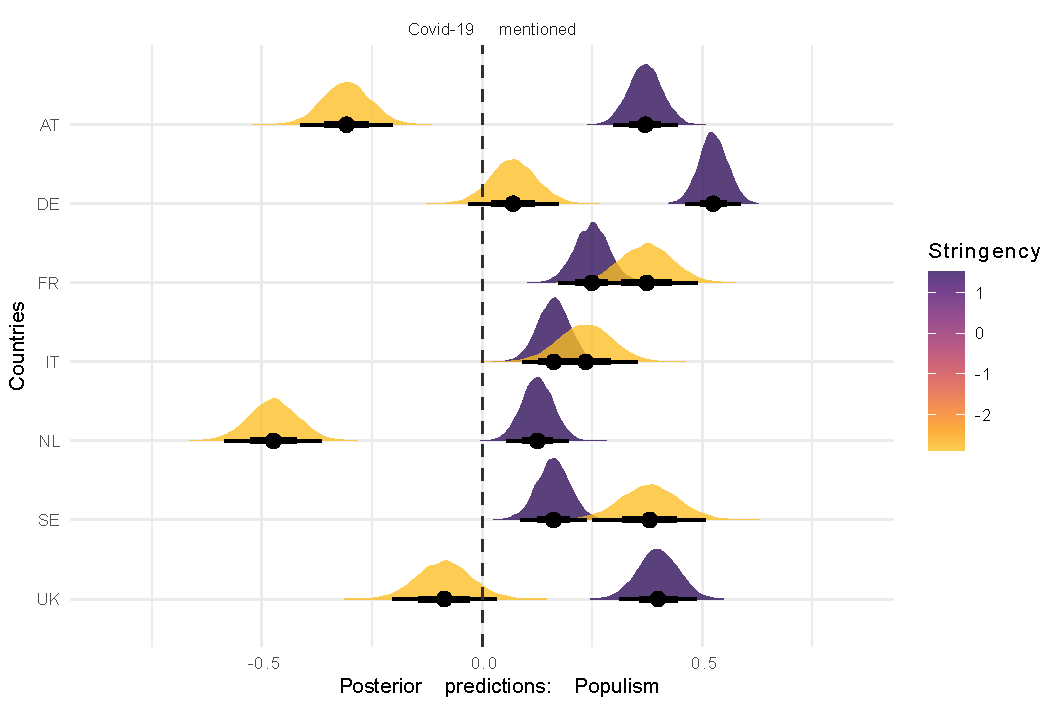
\includegraphics{plots/plot_strgXcov_SEP_ctry_fxdeff_20231130.pdf}

}

\caption{Conditional effects of stringency on the predicted level of
populism by country}

\end{figure}



\end{document}
